% =========================================================================== %
% One Day Tutorial
% =========================================================================== %

\ifx\wholebook\relax\else
  \documentclass[a4paper,10pt,twoside]{book}
  %=============================================================================%
% Common things, settings, packages to include
%=============================================================================%

\usepackage{graphicx}
\usepackage{color}
\usepackage{makeidx}
\usepackage{ifpdf}
\usepackage{verbatim}

% --------------------------------------------------------------------------- %
% Setting up stuff depeding on output format
% --------------------------------------------------------------------------- %

\ifpdf
  % special settings for pdf mode
  \usepackage[colorlinks]{hyperref}
  \usepackage{courier}
  
  \hypersetup{
    colorlinks,
    linkcolor=darkblue,
    citecolor=darkblue,
    pdftitle={The Eclipse Scout Book},
    pdfauthor={The Scout Community},
    pdfkeywords={Enterprise Framework, Eclipse, Java, Client-Side, Rich Client, Web Client, Mobile},
    pdfsubject={Computer Science}
  }
  
  \usepackage{caption}
  \captionsetup{margin=10pt,font=small,labelfont=bf}
\else
  % special stuff for html mode
  \usepackage[tex4ht]{hyperref}
\fi

% --------------------------------------------------------------------------- %
% Setting up printing range
% --------------------------------------------------------------------------- %

\parindent 1cm
\parskip 0.2cm
\topmargin 0.2cm
\oddsidemargin 1cm
\evensidemargin 0.5cm
\textwidth 15cm
\textheight 21cm

% --------------------------------------------------------------------------- %
% Setting up listings
% --------------------------------------------------------------------------- %

\usepackage{listings}
 
\definecolor{darkviolet}{rgb}{0.5,0,0.4}
\definecolor{darkgreen}{rgb}{0,0.4,0.2} 
\definecolor{darkblue}{rgb}{0.1,0.1,0.9}
\definecolor{darkgrey}{rgb}{0.5,0.5,0.5}
\definecolor{lightblue}{rgb}{0.4,0.4,1}
\definecolor{lightgray}{rgb}{0.97,0.97,0.97}

\renewcommand{\lstlistlistingname}{List of Listings}

% general settings
\lstset{
  basicstyle=\small\ttfamily,
  columns=fullflexible,
  breaklines=true,
  breakindent=10pt,
  prebreak=\mbox{{\color{blue}\tiny$\searrow$}},
  postbreak=\mbox{{\color{blue}\tiny$\rightarrow$}},
  showstringspaces=false,
  backgroundcolor=\color{lightgray}
}

% settings for xml files
\lstdefinelanguage{xml}
{
  commentstyle=\color{darkgrey}\upshape,
  morestring=[b]",
  morestring=[s]{>}{<},
  morecomment=[s]{<?}{?>},
  stringstyle=\color{black},
  identifierstyle=\color{darkblue},
  keywordstyle=\color{cyan},
  morekeywords={xmlns,name,point,factory,class}% list your attributes here
}

% settings for ini files
\lstdefinelanguage{ini}
{
  morecomment=[f][\color{darkgrey}\upshape][0]\#, % # is comment iff it's the first char on the line
  stringstyle=\color{black}
}

% default settings (for java files)
\lstset{
  language=Java,
  emphstyle=\color{red}\bfseries,
  keywordstyle=\color{darkviolet}\bfseries,
  commentstyle=\color{darkgreen},
  morecomment=[s][\color{lightblue}]{/**}{*/},
  stringstyle=\color{darkblue},
}

% --------------------------------------------------------------------------- %
% cross reference macros
% --------------------------------------------------------------------------- %
\newcommand{\applabel}[1]{\label{apx:#1}}
\newcommand{\chalabel}[1]{\label{cha:#1}}
\newcommand{\seclabel}[1]{\label{sec:#1}}
\newcommand{\lstlabel}[1]{\label{lst:#1}}
\newcommand{\figlabel}[1]{\label{fig:#1}}
\newcommand{\tablabel}[1]{\label{tab:#1}}

\newcommand{\appref}[1]{Appendix~\ref{apx:#1}}
\newcommand{\charef}[1]{Chapter~\ref{cha:#1}\xspace}
\newcommand{\secref}[1]{Section~\ref{sec:#1}}
\newcommand{\lstref}[1]{Listing~\ref{lst:#1}\xspace}
\newcommand{\figref}[1]{Figure~\ref{fig:#1}\xspace}
\newcommand{\tabref}[1]{Table~\ref{tab:#1}\xspace}

% --------------------------------------------------------------------------- %
% graphics paths
% --------------------------------------------------------------------------- %
\graphicspath{
  {figures/}
  {Introduction/figures/}
}

%=============================================================================%

  \pagestyle{headings}
  \graphicspath{{figures/} {../figures/}}
  \begin{document}
  \sloppy
\fi

% --------------------------------------------------------------------------- %
\chapter{A Larger Example}
\chalabel{large_example}

In this chapter we will create the ''My Contacts'' Scout application.
This small\footnote{
Small in comparison with real world application. But significantly larger and complexer than the ''Hello World'' application of \charef{helloworld}.
} application covers additional aspects of the Eclipse Scout framework. 
The presented demo application borrows heavily from a Scout tutorial published in 2012 the German \textit{Java Magazin}\footnote{
Java Magazin 7.12: \url{https://jaxenter.de/magazines/JavaMagazin72012}.
} 
for the Scout release 3.8 (Juno).
Compared to the 2012 tutorial, the version presented in this chapter has been slightly polished and updated to the Scout release 3.9 (Kepler).

Specifically, we will build an outline based Scout application featuring a navigation tree and pages to present information in tabular form. 
In addition, the application also shows how to work with forms to enter and/or update data, menus and context menus. 
On the server side, we show how to work with databases, how to use logging in Scout applications and how to include standard Java libraries available in JAR files. 

The chapter is organized as follows.
In the first section, the finished demo application is explained from the user perspective. 
The remaining sections focus on the individual steps to implement the ''My Contacts'' application. 
To follow the description of the implementation the reader is assumed to be familiar with the ''Hello World'' tutorial and the Scout SDK as described in \charef{tooling}. 

% --------------------------------------------------------------------------- %
\section{The ''My Contacts'' Application}
\seclabel{my_contacts_guide}

The ''My Contacts'' application is a client server application to manage personal contacts. 
Persistence of entered data is achieved through a database backend. 

As social networking services\footnote{
Social networking services in Wikipedia: \url{http://en.wikipedia.org/wiki/Social_network_service}
} 
such as Facebook, LinkedIn or Xing are widely used, the application also provides an example integration with the LinkedIn\footnote{
\url{http://www.linkedin.com/}
} 
platform. 
The implemented integration allows to download the personal contacts into the local database. 
In the local database it is possible to mix persons entered manually with contact data downloaded from LinkedIn. 

\begin{figure}
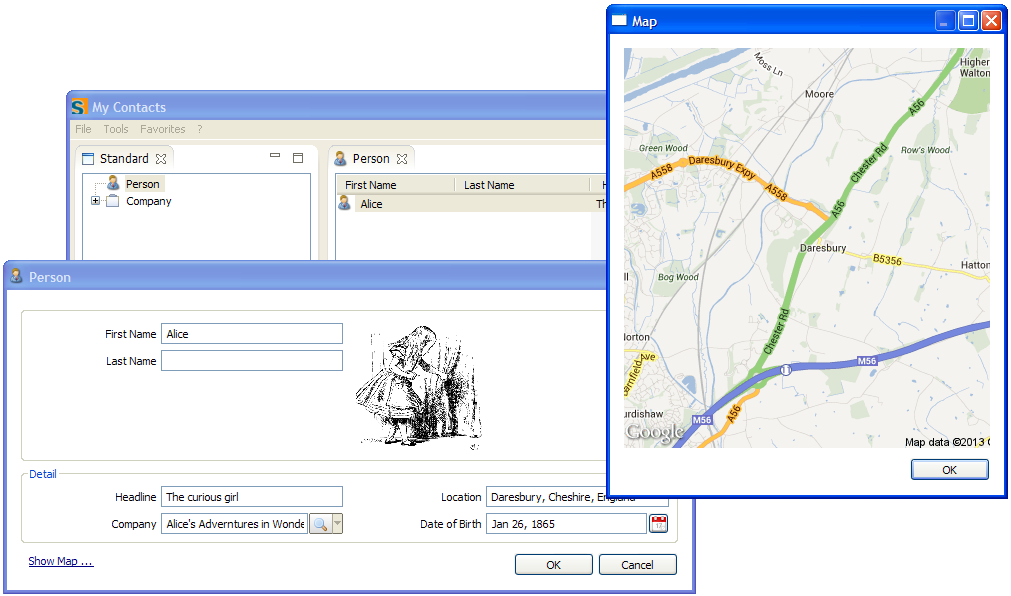
\includegraphics[width=15cm]{my_contacts_swt.png} 
\caption{The SWT client of the ''My Contacts'' application. }
\figlabel{my_contacts_swt}
\end{figure}

After starting the Scout server application a client application may be started that then connects to the server. 
In \figref{my_contacts_swt} the SWT desktop client is shown. 
In the background, the main application window is visible showing a navigation tree on the left hand side. 
On the right side, a table holds the elements corresponding to the selected tree node. 
Using an edit context menu on the selected table row, a form to edit the relevant data may be opened as shown in the example screen shot for 'Alice'. 
Clicking on the link 'Show Map ...' in the person form opens the person's location information in a map form using the data provided by Google Maps Image API\footnote{
The Google Maps Image APIs: \url{https://developers.google.com/maps/documentation/imageapis/}.
}.

\begin{figure}
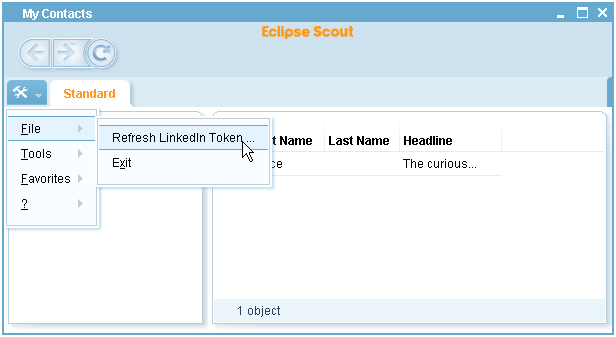
\includegraphics[width=9cm]{my_contacts_rayo_refresh.png} 
\caption{To refresh/generate an access token for reading LinkedIn contacts data select the menu shown in the screen shot. }
\figlabel{my_contacts_rayo_refresh}
\end{figure}

\begin{figure}
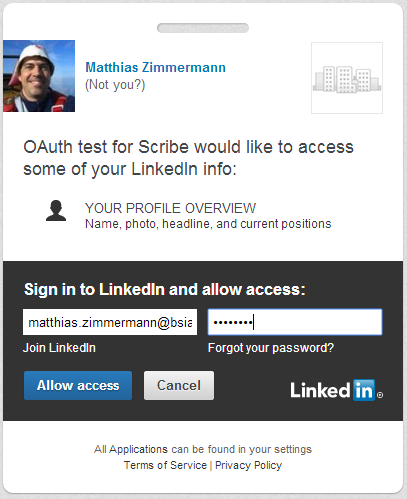
\includegraphics[width=7cm]{my_contacts_rayo_openauthurl.png} \hspace{5mm}
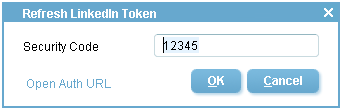
\includegraphics[width=7cm]{my_contacts_rayo_entercode.png}
\caption{To refresh/create the access token click on the provided 'Open Auth URL' link first (left). 
Then, the security code field is enabled and the user can fill in the security code provided on the LinkedIn web page. }
\figlabel{my_contacts_rayo_openauthurl}
\end{figure}

Before any LinkedIn data can be accessed from the ''My Contacts'' application an access token needs to be retrieved from LinkedIn. 
To obtain such a token use the \menu{Refresh LinkedIn Token ...} as shown in \figref{my_contacts_rayo_refresh}. 
This opens the refresh token form shown on the left side of \figref{my_contacts_rayo_openauthurl}. 

\begin{figure}
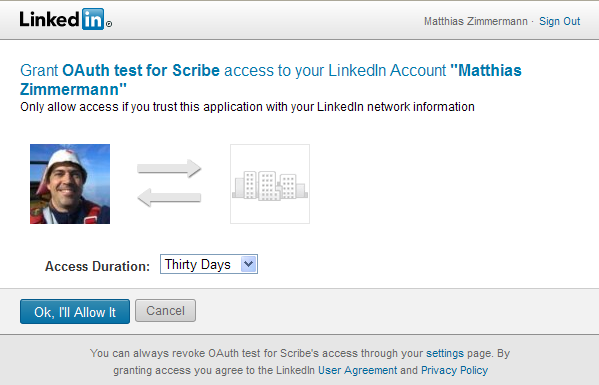
\includegraphics[width=7cm]{oauth_grant_access.png} \hspace{5mm}
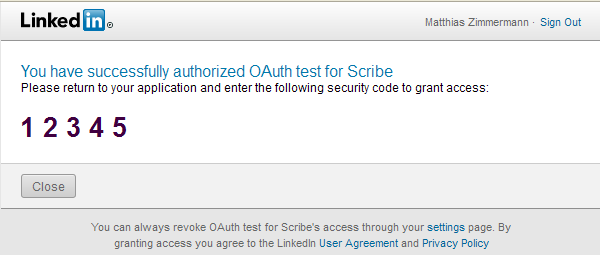
\includegraphics[width=7cm]{oauth_security_code.png} 
\caption{The LinkedIn granting dialog steps shown in a web browser. 
In the first step (right) confirm the access request, then the security code to create an access token is provided in the second step (left).
}
\figlabel{oauth_security_code}
\end{figure}

Clicking on the 'Open Auth URL' link then opens the granting page provided by LinkedIn shown on the left hand side of \figref{oauth_security_code}. 
After logging into your LinkedIn account\footnote{
Yes, for this use case you need a LinkedIn account. But at least it's free and you will not need to provide very sensitive information such as a mobile phone number, a credit card number or a social security number. 
}
you can specify the desired access duration and confirm the ''OAuth test for Scribe'' access\footnote{
This is the name of the example code provided with the Scribe library that is used with the ''My Contacts'' application. 
} 
to your LinkedIn data.
If the authorization is successful, a security code as shown on the right side of \figref{oauth_security_code} is presented by LinkedIn. 
This code needs then to be entered into the \field{Security Code} as shown on the right side of \figref{my_contacts_rayo_openauthurl}. 
Then, click the \button{OK} to refresh the access token. 

\begin{figure}
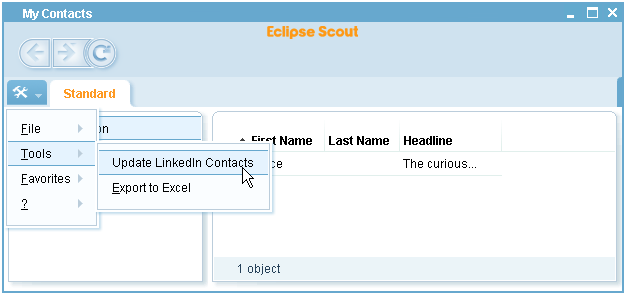
\includegraphics[width=9cm]{my_contacts_rayo_updatecontacts.png} \hspace{5mm}
\caption{Executing the 'Update LinkedIn Contacts for the first time imports the users LinkedIn contacts into the ''My Contacts'' application.}
\figlabel{my_contacts_rayo_updatecontacts}
\end{figure}

To import/update your LinkedIn contacts into your ''My Contacts'' application select the \menu{Update LinkedIn Contacts} as shown in \figref{my_contacts_rayo_updatecontacts}.
Once you have downloaded or entered a number of persons in your ''My Contacts'' application, try to get yourself familiar with the application's person table. 
This is one of the very powerful Scout widgets. 
Columns may be filtered, moved, hidden or sorted (including multi level sort) using the table header context menus \menu{Organize Columns...}  and \menu{Column Filter...}.

Editing and viewing of person data is available by the \contextmenu{Edit Person...} on a selected row.
To manually add a person use the context \contextmenu{New Person...} available on the table header or in the white area outside the displayed columns. 

\begin{figure}
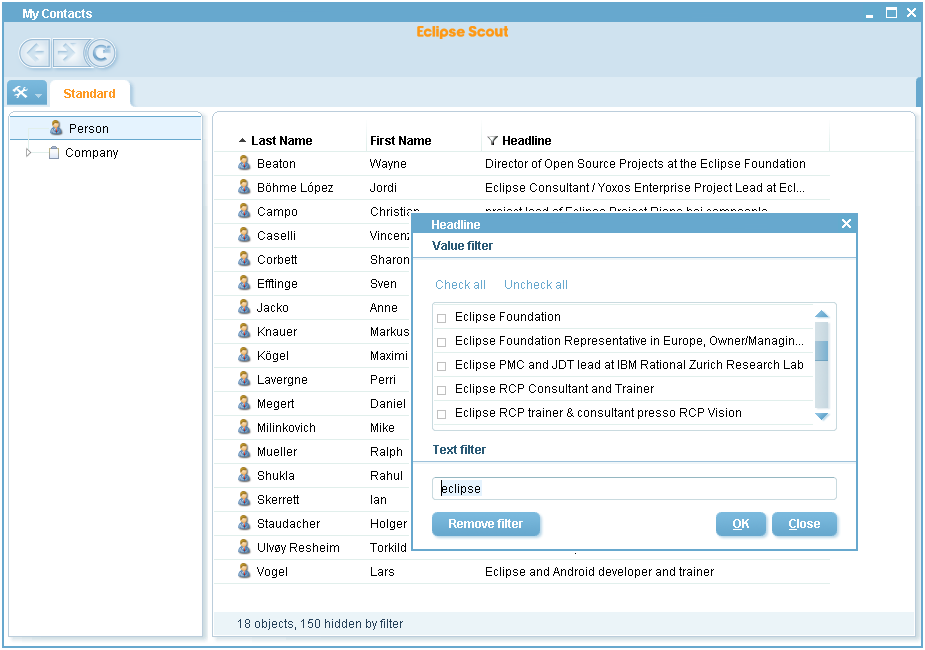
\includegraphics[width=14cm]{my_contacts_rayo_filteredcontacts.png} 
\caption{After importing the contacts from LinkedIn the data is shown in the person page. 
The filter applied on the headline column is indicated by the filter icon. In the front, the filter form shows the filter criteria 'Eclipse'.}
\figlabel{my_contacts_rayo_filteredcontacts}
\end{figure}

\begin{figure}
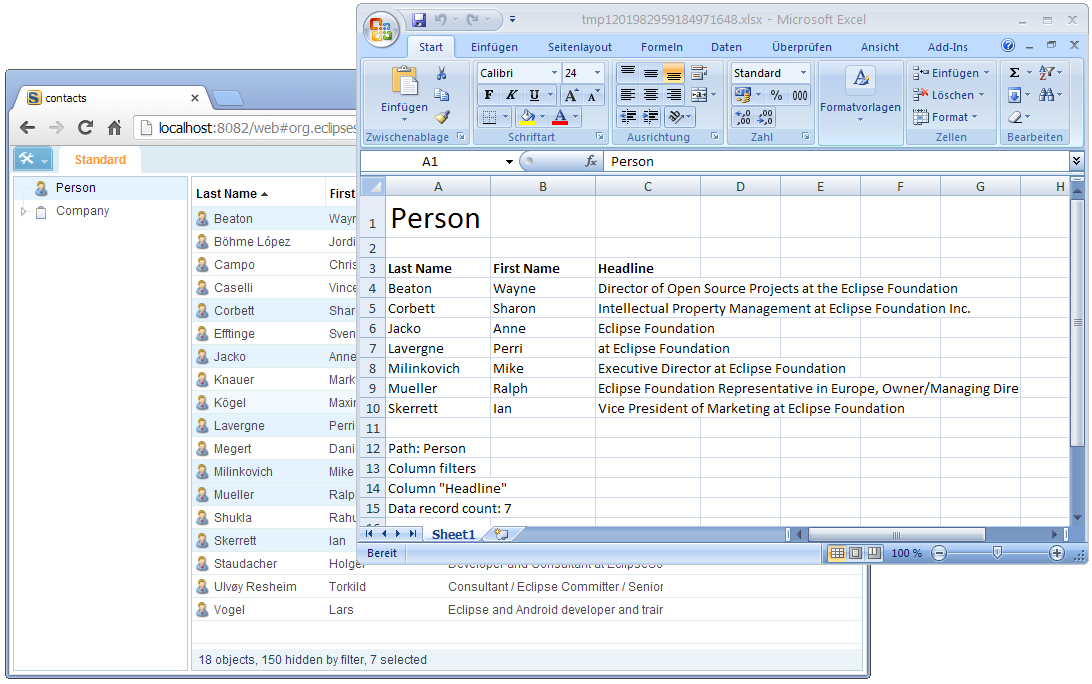
\includegraphics[width=14cm]{my_contacts_rapweb_excelexport.png} 
\caption{The ''My Contacts'' application running in the browser as web application. 
The Excel sheet shown in the front is exported from the person page using the 'Tools/Export to Excel' menu. }
\figlabel{my_contacts_rapweb_excelexport}
\end{figure}

\begin{figure}
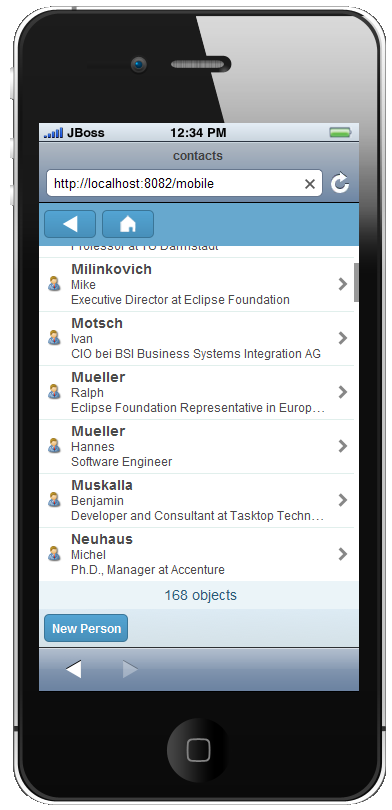
\includegraphics[width=6cm]{my_contacts_rapmobile_1.png} \hspace{5mm}
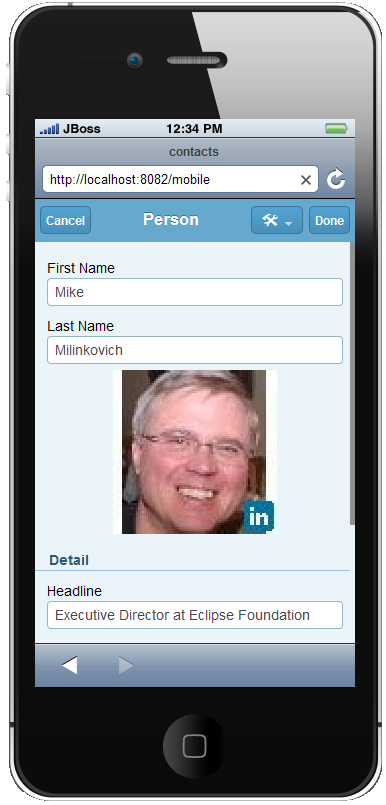
\includegraphics[width=6cm]{my_contacts_rapmobile_2.png} \hspace{5mm}
\caption{The ''My Contacts'' application running on an iPhone device. 
On the left hand side, the person page is shown. The person form is shown on the right. }
\figlabel{my_contacts_rapmobile}
\end{figure}

In \figref{my_contacts_rapweb_excelexport} the ''My Contacts'' application is running in a web browser. 
In this example, the \menu{Tools|Export to to Excel} is used to export the selected row into an Excel sheet. 
Finally, the ''My Contacts'' application is also running on iPhone and Android mobile devices out of the box. 
Two example screens are provided in \figref{my_contacts_rapmobile}.

Once you no longer feel confident about having the ''My Contacts'' application accessing you data you can revoke this access permission in the LinkedIn menu ''Privacy and Settings''. 
In the lower part of the settings page switch to tab ''Groups, Companies and Applications'' and click on the link ''View your applications''. 
There, you will find again the partner name ''OAuth test for Scribe''. 
To revoke the access, select the associated checkbox and click the ''Remove'' button. 
The next time you try to refresh your LinkedIn data from the ''My Contacts'' application will result in an Error message. 
Before you can again access data from your LinkedIn account you just need to refresh the access token as described above.

To run the ''My Contacts'' Scout application without implementing it first, you may take advantage of the fact that the application is hosted in the same Github repository as this book.
If you are familiar with Github\footnote{
Github: \url{https://en.wikipedia.org/wiki/GitHub}.
}, 
fork the Scout Book repository\footnote{
Scout Book repository: \url{https://github.com/BSI-Business-Systems-Integration-AG/scoutbook}.
} 
and start from there.
Alternatively, you can follow the description provided in the Scout wiki\footnote{
Download and installation of the ''My Contacts'' application: \url{http://wiki.eclipse.org/Scout/Book/3.9\#Download_and_Run_the_Scout_Sample_Applications}.
}
to download, install and run the ''My Contacts'' application.

% --------------------------------------------------------------------------- %
\section{Setting up the new Scout project}

\begin{figure}
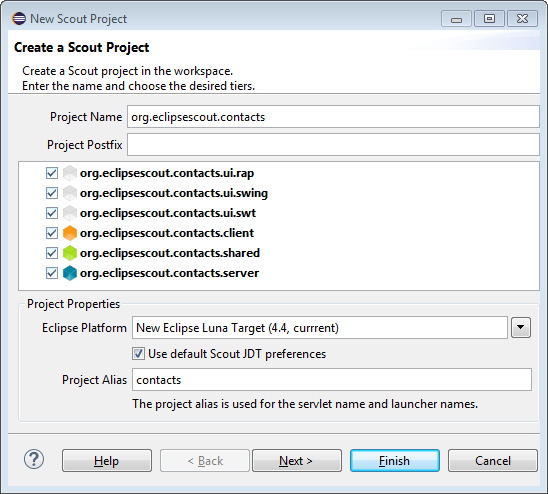
\includegraphics[width=7cm]{new_project_contacts_1.png} \hspace{5mm}
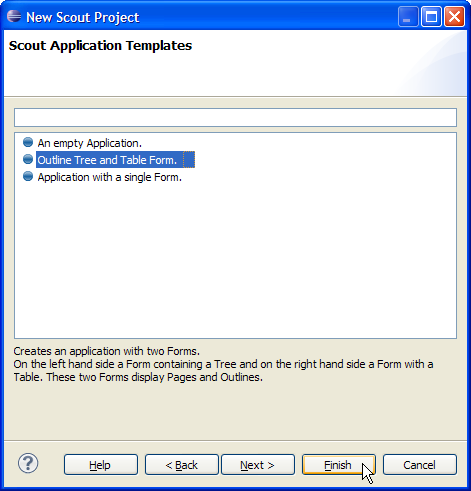
\includegraphics[width=7cm]{new_project_contacts_2.png}
\caption{Start with creating a new Scout project. }
\figlabel{new_project_contacts}
\end{figure}

The initial code for the ''My Contacts'' application is generated using the \wizard{New Scout Project} as described in \secref{wizard_new_project}. 
For the \field{Project Name} use the name \java{org.eclipsescout.contacts} as shown on the left side of \figref{new_project_contacts} and click on the \button{Next}. 
In the second wizard step select the application template \element{Outline Tree and Table Form} as shown on the right side of \figref{new_project_contacts}.

\begin{figure}
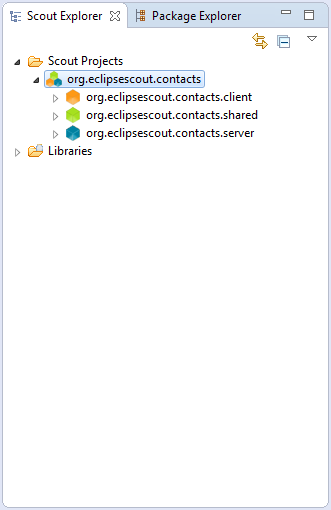
\includegraphics[width=7cm]{project_contacts_explorer.png} \hspace{5mm}
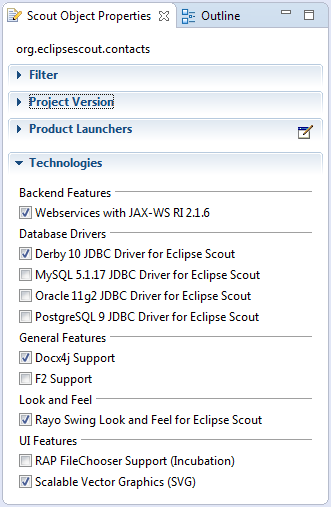
\includegraphics[width=7cm]{project_contacts_properties.png}
\caption{The setting of the \textit{Technology} section in the Scout Object Properties of the ''My Contacts'' application.}
\figlabel{project_contacts_properties}
\end{figure}

After the Scout SDK has created the initial application code select the top-level \node{org.eclipsescout.contacts} in the Scout Explorer. 
In the technology section of the corresponding Scout Object Properties select the Derby database driver, the Docx4j support and the Rayo look and feel as shown on the right side of \figref{project_contacts_properties}.
In case you have not yet used the Scout Docx4j support or the Rayo look and feel components, the Scout SDK will need to download these packages from the Eclipse Marketplace\footnote{
See \secref{scout_sdk_object_properties} for additional information regarding the download of marketplace packages
}
first. 

\lstinputlisting[
  label=\lstlabel{mycontacts.desktop.menu.exportoexcel},
  caption=The \java{ExportToExcelMenu} class added by the Docx4j support to the application's tools menu.,
  index={ScoutXlsxSpreadsheetAdapter,IShellService,shellOpen},
  linerange={145-162},
  float
]
{../code/oneDayTutorial/org.eclipsescout.contacts.client/src/org/eclipsescout/contacts/client/ui/desktop/Desktop.java}

Adding the Docx4j support will also add the \menu{Export to Excel} under tools menu on the application's desktop.
As shown in \lstref{mycontacts.desktop.menu.exportoexcel}, the \java{ScoutXlsxSpreadsheetAdapter} first creates an excel file based on the currently active page in the \java{execAction} method. 
Then the file is opened on the client using the \java{shellOpen} method.

\begin{figure}
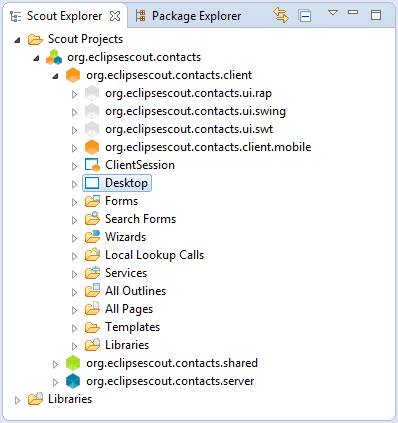
\includegraphics[width=7cm]{desktop_explorer.png} \hspace{5mm}
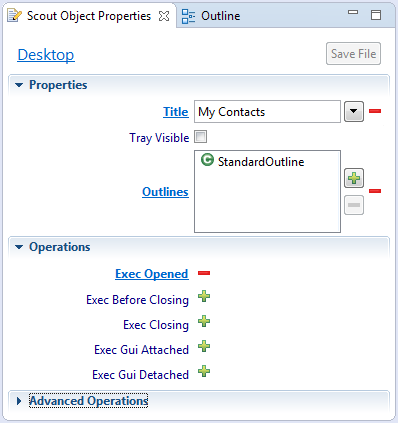
\includegraphics[width=7cm]{desktop_properties.png}
\caption{Configure the application name in the title field of the Desktop's properties. }
\figlabel{desktop_properties}
\end{figure}

To set the applications name select the \node{Desktop} in the Scout Explorer to access it's Scout Object Properties as shown in \figref{desktop_properties}.
In the \field{Title} enter the string ''My Contacts'' create a new translated text entry. 
Then click on the \link{Exec Opened} in the Scout Object Properties to access the Java code of this method. 

\lstinputlisting[
  label=\lstlabel{mycontacts.desktop.execopened},
  caption=The \java{execOpened} method of desktop class of the "My Contacts" application. The application's organisation into a tree and a table form is defined here.,
  index={execOpened,Desktop,UserAgentUtility},
  linerange={49-70},
  float
]
{../code/oneDayTutorial/org.eclipsescout.contacts.client/src/org/eclipsescout/contacts/client/ui/desktop/Desktop.java}

As shown in \lstref{mycontacts.desktop.execopened} the application's organisation into a tree and a table form is explicitly defined in method \java{execOpened}. 
First, using the \java{UserAgentUtility} class, the method checks if the client is working with a desktop or a web client. 
If not, the method returns and not tree and table setup is used. 
Instead, the \java{MobileHomeForm} defined in plugin \element{org.eclipsescout.contacts.client.mobile} is used. 
In case the user is working with a web client or a desktop client, default tree and table forms are created and started. 
Finally, the currently active outline is set to the \java{StandardOutline}, as this is the only outline defined in this application.

% --------------------------------------------------------------------------- %
\section{Adding the Person Page}

\begin{figure}
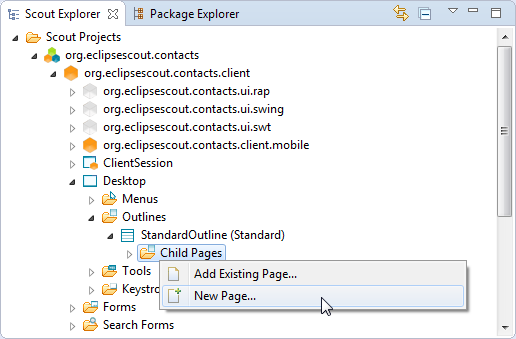
\includegraphics[width=5cm]{new_page_person_contextmenu.png} \hspace{2mm}
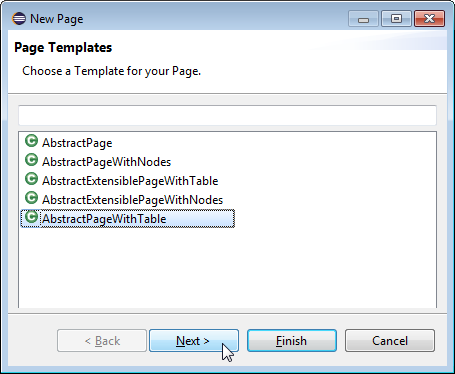
\includegraphics[width=4.5cm]{new_page_person_1.png} \hspace{2mm}
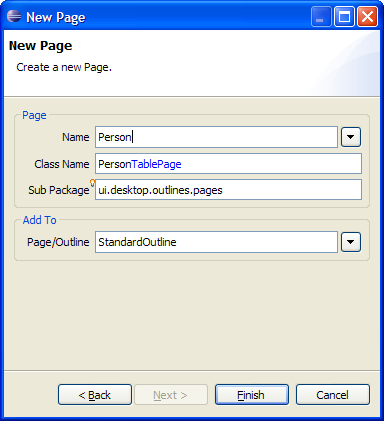
\includegraphics[width=4.5cm]{new_page_person_2.png}
\caption{Add the person table page below the standard outline. }
\figlabel{new_page_person}
\end{figure}

The first UI component we add to the application is the person page. 
For the desktop clients, this page is represented as a table that will list all available persons in the database of the ''My Contacts'' application. 
To start the \wizard{New Page} use the \contextmenu{New Page...} on the \folder{Child Pages} as shown in \figref{new_page_person}.
On the first wizard step select the template \element{AbstractPageWithTable} and click the \button{Next}. 
On the second wizard step, provide the page name ''Person'' to create a new translated text entry at the same time. 
Make sure the other fields are filled in as shown in \figref{new_page_person} and click the \button{Finish} to close the wizard.

\lstinputlisting[
  label=\lstlabel{mycontacts.desktop.outline.personpage},
  caption=The \java{execCreateChildPages} method of the standard outline. At the current implementation step the company table page is not (yet) added.,
  index={execCreateChildPages, StandardOutline},
  linerange={19-25},
  float
]
{../code/oneDayTutorial/org.eclipsescout.contacts.client/src/org/eclipsescout/contacts/client/ui/desktop/outlines/StandardOutline.java}

\lstref{mycontacts.desktop.outline.personpage} shows the created method \java{execCreateChildPages} that links the newly created person page to the standard outline. 
Note that your code will only look the same once you have added the company page in a later step of the implementation of this application.

\begin{figure}
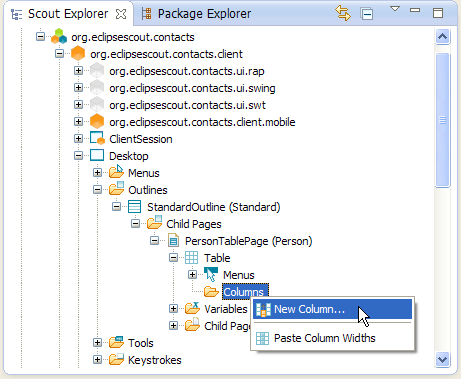
\includegraphics[width=5cm]{new_column_personid_contextmenu.png} \hspace{2mm}
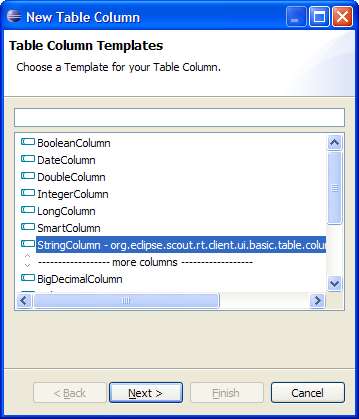
\includegraphics[width=4.5cm]{new_column_personid_1.png} \hspace{2mm}
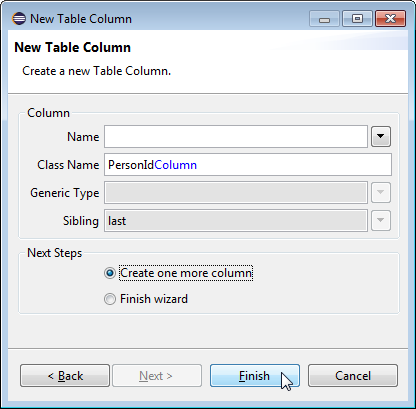
\includegraphics[width=4.5cm]{new_column_personid_2.png}
\caption{Add columns to the person page.}
\figlabel{new_column_personid}
\end{figure}

Now, drill down to the \folder{Columns} under the \node{PersonTablePage} as shown in \figref{new_column_personid}. 
Here we can add the desired table columns to the person page. 
Start with the column that will hold the person id. 
For this, start the column wizard as shown on the left side of \figref{new_column_personid} and select the string column template. 
In the second wizard step, enter ''PersonId'' into the \field{Class Name},select the radio button \element{Create one more column} and click on the \button{Finish}. 
This will restart the column wizard to enter the next columns. 
Create the remaining string columns with the following names.

\begin{itemize}
  \item{First Name}
  \item{Last Name}
  \item{Headline}
\end{itemize}

\begin{figure}
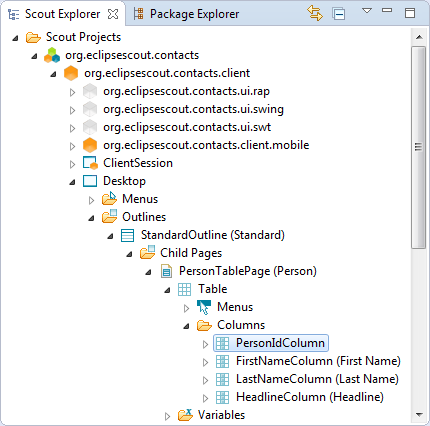
\includegraphics[height=7cm]{person_id_column.png} \hspace{5mm}
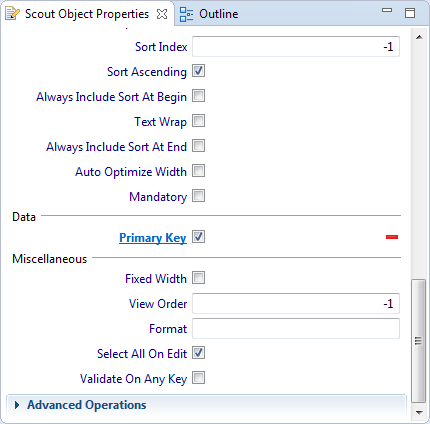
\includegraphics[height=7cm]{person_id_property.png}
\caption{Configure the \element{PersonId} column. Check property \element{Primary Key} under the section \element{Advanced Properties} (right).}
\figlabel{new_column_personid}
\end{figure}

\lstinputlisting[
  label=\lstlabel{mycontacts.desktop.outline.personpage.columns},
  caption=The person id and the first name columns of the \java{PersonTablePage} class. ,
  index={A primary key table column and a default string column.},
  linerange={71-93},
  float
]
{../code/oneDayTutorial/org.eclipsescout.contacts.client/src/org/eclipsescout/contacts/client/ui/desktop/outlines/pages/PersonTablePage.java}

Once you have created all these columns we will mark the person id column as the primary key column for the person page. 
In the Scout Explorer select the \node{PersonIdColumn} to open the corresponding Scout Object Properties. 
In this form, deselect the \property{Displayable} to always hide this technical column from the end user. 
In the properties \element{Advanced Properties} section check the \property{Primary Key}. 
The resulting Java code for the primary key column and the first name column is provided in \lstref{mycontacts.desktop.outline.personpage.columns}. 

\begin{figure}
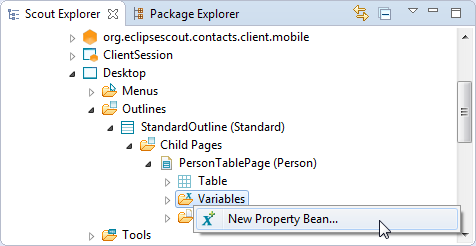
\includegraphics[height=5cm]{new_bean_companyid_contextmenu.png} \hspace{5mm}
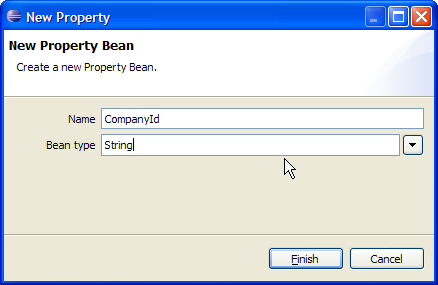
\includegraphics[height=5cm]{new_bean_companyid.png}
\caption{Add the \element{CompanyId} variable to the person page.}
\figlabel{new_bean_companyid}
\end{figure}

\lstinputlisting[
  label=\lstlabel{mycontacts.desktop.outline.personpage.columns},
  caption=The company id variable of the \java{PersonTablePage} class. ,
  index={A table page property bean.},
  linerange={18-21,162-172},
  float
]
{../code/oneDayTutorial/org.eclipsescout.contacts.client/src/org/eclipsescout/contacts/client/ui/desktop/outlines/pages/PersonTablePage.java}

As we will later add and link the person page with a company page, we add a company id variable to the person page as shown in \figref{new_bean_companyid}. 
For the Java representation of such variables the standard bean pattern is used as shown in \lstref{mycontacts.desktop.outline.personpage.columns}.

% --------------------------------------------------------------------------- %
\section{Adding the Company Page}

\begin{figure}
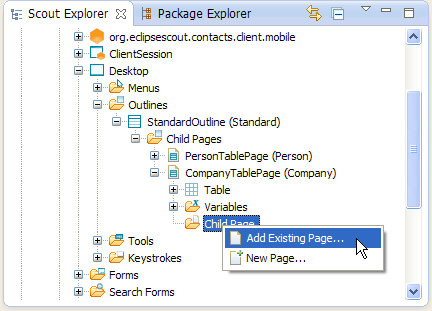
\includegraphics[width=6.5cm]{add_existing_page_contextmenu.png} \hspace{5mm}
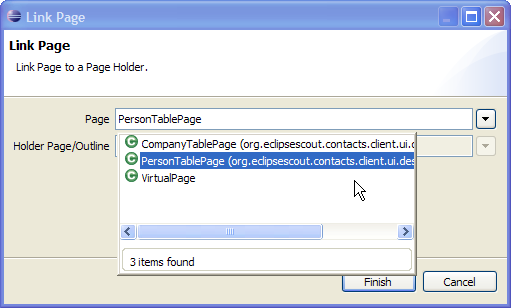
\includegraphics[width=7.5cm]{add_existing_page.png}
\caption{Add the person page below the the company page.}
\figlabel{add_existing_page}
\end{figure}

\lstinputlisting[
  label=\lstlabel{mycontacts.desktop.outline.companypage.linking},
  caption=Linking the \java{PersonTablePage} with the parent \java{CompanyTablePage}.,
  index={Linking pages hierarchically.},
  linerange={30-36},
  float
]
{../code/oneDayTutorial/org.eclipsescout.contacts.client/src/org/eclipsescout/contacts/client/ui/desktop/outlines/pages/CompanyTablePage.java}

After adding the person page, we add a company page to the standard outline. 
To add the company page we use the same wizards as described in the previous section for the person page. 
For the \field{Name} we enter the new translated text ''Company'' and the columns to add are the following.

\begin{itemize}
  \item{Company Id}
  \item{Name}
  \item{Location}
\end{itemize}

As in the case of the person table page, the company id column is used as a primary key column. 
The \property{Displayable} needs to be set to false and the \property{Primary Key} to true. 
Now we can link the person page to the company page using the \contextmenu{Add Existing Page...} as shown on the left side of \figref{add_existing_page}. 
In the \wizard{Link Page}, the person page can then be selected according to the right side of \figref{add_existing_page}. 
In the Java code generated by the Scout SDK the setting of the company id attribute is automatically inserted in method \java{execCreateChildPages}. 
Please note that this convenience added by the Scout SDK wizard only works if the child page defines variables with a naming that matches the defined primary key columns of the parent table. 

% --------------------------------------------------------------------------- %
\section{Installing the Database}

\begin{figure}
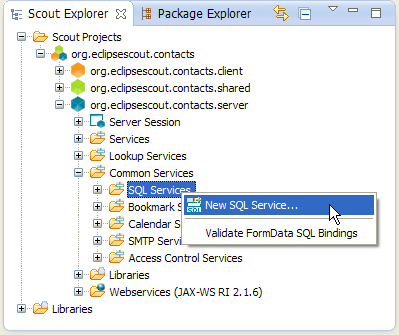
\includegraphics[width=7cm]{new_service_derby_contextmenu.png} \hspace{5mm}
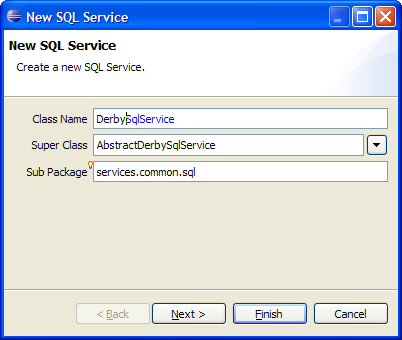
\includegraphics[width=7cm]{new_service_derby.png} 
\caption{Add the service to access the Derby database under folder \element{SQL Services}. }
\figlabel{new_service_derby}
\end{figure}

To access a database we first need to install a database service. 
For the ''My Contacts'' application, this is done using the \wizard{New SQL Service} on the Scout server under the \folder{SQL Services} as shown in \figref{new_service_derby}.
In the first wizard step shown on the right side of the figure, use ''DerbySqlService'' for the \field{Class Name}.
From the drop-down list in the \field{Super Class} choose the \java{AbstractDerbySqlService} and click on the \button{Finish}.

\lstinputlisting[
  label=\lstlabel{mycontacts.server.configini.derby},
  caption=Setting up the database parameters in the Scout server's \texttt{config.ini} file.,
  index={database setup, config.ini},
  linerange={42-48},
  float
]
{../code/oneDayTutorial/org.eclipsescout.contacts.server/products/development/config.ini}

To setup the database connection the necessary parameters need to be added to the server's \filename{config.ini} file as shown in \lstref{mycontacts.server.configini.derby}.
Comparing the parameter names in this config file with the package name of the created \java{DerbySqlService} service class reveals an interesting framework feature. 
All Scout services can be parameterized using the \filename{config.ini} file with the pattern \java{<package>.<class name>\#<parameter>=<value>}. 
The Scout runtime then sets the service parameters using matching setter methods such as \java{setPassword} for the password parameter.  

According to the parameter \java{jdbcMappingName=jdbc:derby:\$\{workspace\_loc\}/...} a new Derby database will be created in the same parent directory as the ''My Contacts'' workspace directory if no database named \java{DB\_CONTACT} is found there.
This setup is handy for development purposes but you may want to set the database parameter to \java{create=false} in the \filename{config.ini} of the production product file. 

\begin{figure}
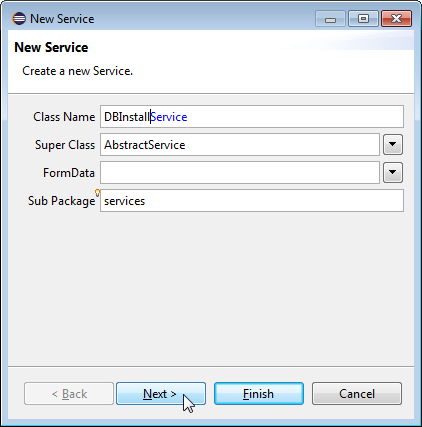
\includegraphics[width=7cm]{new_service_dbinstall_1.png} \hspace{5mm}
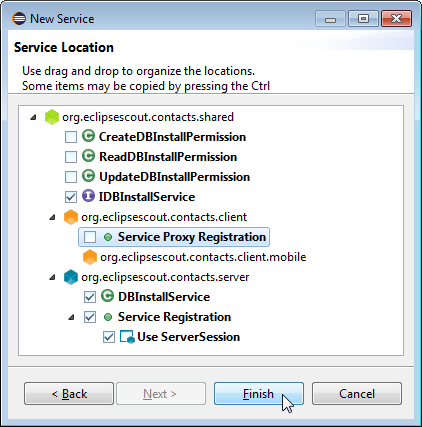
\includegraphics[width=7cm]{new_service_dbinstall_2.png} 
\caption{Add a database installation service. }
\figlabel{new_service_dbinstall}
\end{figure}

\begin{figure}
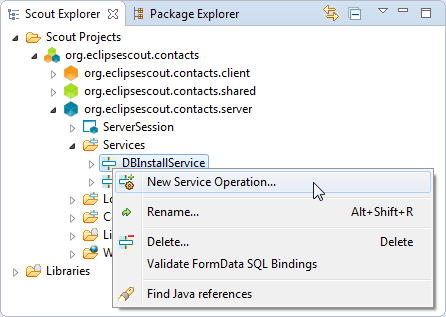
\includegraphics[height=5.5cm]{new_operation_installstorage_contextmenu.png} \hspace{5mm}
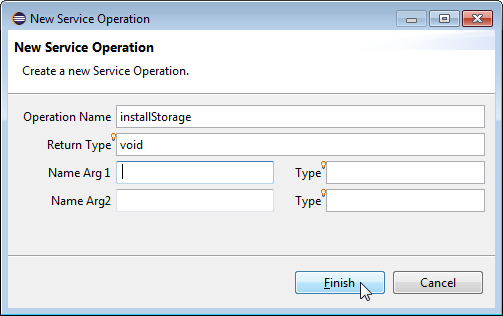
\includegraphics[height=5.5cm]{new_operation_installstorage.png} 
\caption{Add the service operation to create the DB schema. }
\figlabel{new_operation_installstorage}
\end{figure}


\lstinputlisting[
  label=\lstlabel{mycontacts.server.services.installdb},
  caption=The \java{installStorage} service operation to create the database schema for the ''My Contacts'' application.
  New tables are created if they are not found by \java{getExistingTables} in the existing schema.,
  index={A service operation to install a database schema.},
  linerange={14-16,21-36,94-105},
  float
]
{../code/oneDayTutorial/org.eclipsescout.contacts.server/src/org/eclipsescout/contacts/server/services/DBInstallService.java}

% ........................................................................... %
\subsection{Setting up the Database Schema}

Having a working database service and a new (empty) Derby database now allows to create the necessary database schema and populate it with some initial data.
For this we add a new \java{DBInstallService} service as shown in \figref{new_service_dbinstall}.
To this install service we then add the \java{installStorage} operation according to \figref{new_operation_installstorage}.
The implementation of this method is provided in \lstref{mycontacts.server.services.installdb}.
The method first checks if a setup is required. 
For this, the member variable \java{m\_doSetup} is used that might also be set by the \java{setDoSetup} setter method via the server's the \filename{config.ini} file.

\lstinputlisting[
  label=\lstlabel{mycontacts.server.services.installdb.company},
  caption=Setting up the \java{COMPANY} table of the ''My Contacts'' application.,
  linerange={37-56},
  float
]
{../code/oneDayTutorial/org.eclipsescout.contacts.server/src/org/eclipsescout/contacts/server/services/DBInstallService.java}

\lstinputlisting[
  label=\lstlabel{mycontacts.server.services.installdb.person},
  caption=Setting up the \java{PERSON} table of the ''My Contacts'' application.,
  linerange={57-79},
  float
]
{../code/oneDayTutorial/org.eclipsescout.contacts.server/src/org/eclipsescout/contacts/server/services/DBInstallService.java}

\lstinputlisting[
  label=\lstlabel{mycontacts.server.services.installdb.users_param},
  caption=Setting up the \java{USERS\_PARAM} table of the ''My Contacts'' application.,
  linerange={80-94},
  float
]
{../code/oneDayTutorial/org.eclipsescout.contacts.server/src/org/eclipsescout/contacts/server/services/DBInstallService.java}

Setting up the schema to contain the individual tables for the ''My Contacts'' application is implemented in a separate method per table. 
The table definition for the company table is provided in \lstref{mycontacts.server.services.installdb.company}. 
In this method two Scout aspects are of interest. 

The first Scout feature used is the absence of a \java{COMMIT} statement after the two \java{INSERT INTO} statements. 
This is possible, as all Scout service calls run in a transaction context that is transparent to the Scout developer. 
If a service method exits without errors, the enclosing transaction is committed. 
And if any runtime exception occurs in a service call the Scout runtime framework performs a rollback.

The second feature is the parameter binding used in the \java{INSERT INTO} statements. 
When SQL statements are executed using any of the static \java{SQL} methods, an internal statement processor replaces all bind variables found in the provided statement string. 
In Scout, SQL bind variables need to use the pattern \java{:<variable name>}. 
The values for the bind variables can then be provided in the form of additional arguments. 
In the concrete example of \lstref{mycontacts.server.services.installdb.company}, the content for the bind variable \java{:company\_id} is provided as a \java{NVPair} object. 
\element{NVPair}s are the simplest possible form to represent bind variables. 
The first constructor argument is the variable name of the bind variable, in this case \java{company\_id}. 
The actual content of the bind variable is provided in the form of an object. 
Here, the Java runtime class \java{UUID.randomUUID().toString()} is used to create a new company key. 

Setting up the person table and the user parameter table is defined according to \lstref{mycontacts.server.services.installdb.person} and \lstref{mycontacts.server.services.installdb.users_param}. 
To create a data object for the persons day of birth, the Scout utility class \java{DateUtility} is used.

\lstinputlisting[
  label=\lstlabel{mycontacts.server.serverapplication},
  caption=Scheduling the database installation in the \java{start} method of the \java{ServerApplication} class during the server application startup.,
  index={ServerApplication, ServerSession},
  linerange={30-57,62-63},
  float
]
{../code/oneDayTutorial/org.eclipsescout.contacts.server/src/org/eclipsescout/contacts/server/ServerApplication.java}

The only piece missing to setup the database is calling the \java{installStorage} operation during the startup of the ''My Contacts'' server application.
The proper way to implement such a scenario is to schedule an installation job in the \java{ServerApplication} class of the Scout server. 
In the ''My Contacts'' application this is implemented according to \lstref{mycontacts.server.serverapplication}. 
To create a server job, a new server session object needs to be obtained first. 
However, during the startup time of the server we do not have any logged in users yet. 
That is why the session is created for the backend subject representing the server application. 
Using this \java{serverSession} object, the \java{installJob} can be created. 
In it's \java{runTransaction} method we can then call the \java{installStorage} operation to setup the ''My Contacts'' database.

% ........................................................................... %
\subsection{Scout Logging}

\lstinputlisting[
  label=\lstlabel{mycontacts.server.configini.logging},
  caption=The logging configuration in the Scout server's \texttt{config.ini} file.,
  index={config.ini, logging setup},
  linerange={14-17},
  float
]
{../code/oneDayTutorial/org.eclipsescout.contacts.server/products/development/config.ini}

An additional Scout topic that is touched in this \java{ServerApplication} class is the Scout logging. 
As shown in \lstref{mycontacts.server.serverapplication}, a static \java{logger} object is created using Scout's \java{ScoutLogManager} class. 
Events can then be logged with the \java{logger.info} method where \java{info} refers to the log level attached to this message. 
Similar to the database setup described above, the logging setup can be defined in \filename{config.ini} file. 
The default setup defined for the development product is provided in \lstref{mycontacts.server.configini.logging}.
Further information regarding logging in Eclipse Scout is available in the Scout wiki\footnote{
Logging in Eclipse Scout: \url{http://wiki.eclipse.org/Scout/Concepts/Logging}.
}.

% --------------------------------------------------------------------------- %
\section{Fetching Data from the Database}

\begin{figure}
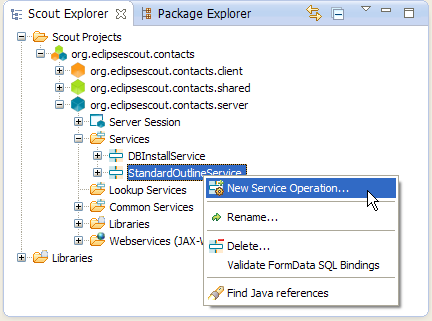
\includegraphics[height=5cm]{new_service_persontabledata_contextmenu.png} \hspace{5mm}
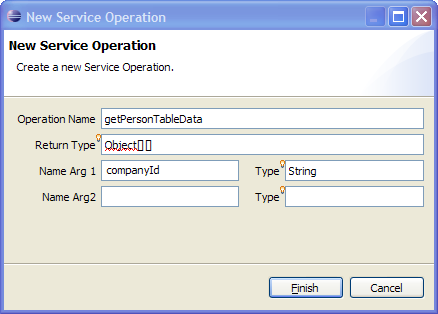
\includegraphics[height=5cm]{new_service_persontabledata.png}
\caption{Add the service operation to fetch the data for the person table. }
\figlabel{new_service_persontabledata}
\end{figure}

In the section before, we have implemented the access to the Derby database for the Scout server. 
And during the server startup, the application's database schema can now be created and populated with some initial data. 

Here, this schema and the implemented database access is used to fetch the data for the client application's person page and the company page. 
The best place to implement these data provider methods is in the server's \java{StandardOutlineService} class. 
This class has been created by the Scout SDK during the initial project creation step.
It is meant to hold the operations that fetch the data for populating the elements visible in the outline tree and outline pages. 

For the ''My Contacts'' application, we first create the \java{getPersonTableData} operation as shown in \figref{new_service_persontabledata}. 
In the wizard dialog enter ''getPersonTableData'' into the \field{Operation Name}. 
For the return type we simply use a two dimensional object array. 
As the person page is also displayed under the company page, we need to have a way to only return the persons working for a specific company. 
To allow for this use case, we add the parameter ''companyId'' as the first argument to the \java{getPersonTableData} operation before we close the wizard with \button{Finish}. 

The next operation we need is the \java{getCompanyTableData} method. 
You may use the same creation steps as described above for the person table page data. 
But for fetching company table data we do not need an additional argument.
The company page in the ''My Contacts'' application will always show all available companies. 

\lstinputlisting[
  label=\lstlabel{mycontacts.server.services.standardoutline},
  caption=Fetching the table data for the person and the company page of the ''My Contacts'' application.
  The list of persons is restricted to employees of a specific company if a company id parameter is provided.,
  index={SQL, StringUtility, bind variables, NVPair, StandardOutlineService},
  linerange={10-29},
  float
]
{../code/oneDayTutorial/org.eclipsescout.contacts.server/src/org/eclipsescout/contacts/server/services/StandardOutlineService.java}

For the actual implementation of the two data fetching operations the code provided in \lstref{mycontacts.server.services.standardoutline} is used. 
The implementation is straight forward and almost trivial. 
However, we can use the \java{getPersonTableData} example to introduce one of the many Scout utility classes. 

\begin{figure}
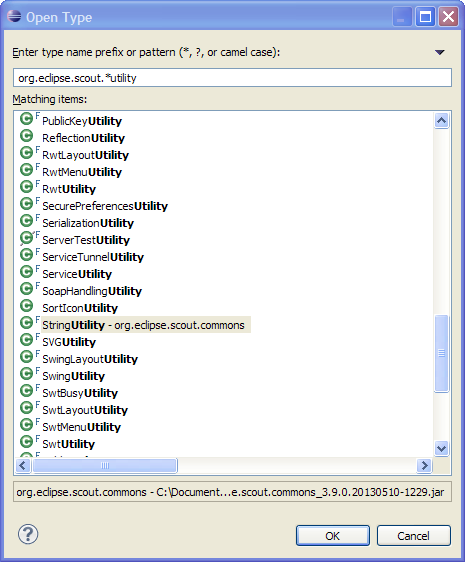
\includegraphics[width=8cm]{scout_utility_classes.png}
\caption{Accessing the Scout utility classes with the pattern \java{org.eclipse.scout.*Utility}.}
\figlabel{scout_utility_classes}
\end{figure}

The class \java{StringUtility} is one of the many utility classes provided by the Scout framework. 
Here, it is used for the typical null or empty check. 
To get a quick overview, hit the \key{Ctrl}\key{Shift}\key{T} key combination. 
In the type dialog that appears enter \java{org.eclipse.scout.*Utility} into the pattern field. 
This will display the complete list of the Scout utility classes as shown in \figref{scout_utility_classes}.

% --------------------------------------------------------------------------- %
\section{Creating the Person Form}

\begin{figure}
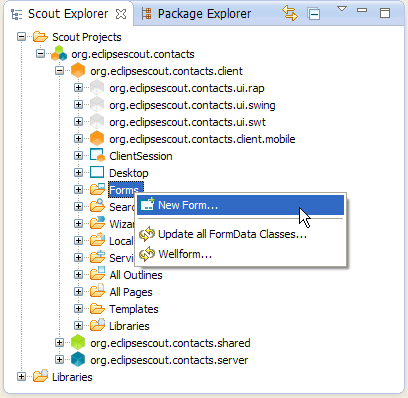
\includegraphics[height=7cm]{new_form_person_contextmenu.png} \hspace{5mm}
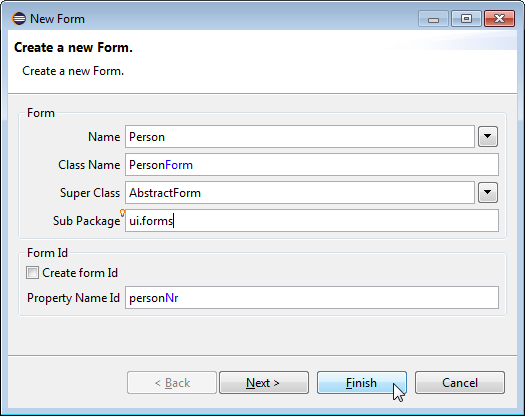
\includegraphics[height=7cm]{new_form_person.png}
\caption{Add the person form.}
\figlabel{new_form_person}
\end{figure}

In this section we will create the person form that is used to display and edit the persons stored in the ''My Contacts'' application. 
To add the person form use the Scout SDK \wizard{New Form} as shown in \figref{new_form_person}. 
In the first wizard step you just need to enter ''Person'' as a new translated text into the \field{Name} and add ''ui.forms'' as the sub-package name in the corresponding wizard field. 
Then click the \button{Finish}.

The wizard will create the necessary artefacts in the application's client, the shared and the server plugin projects. 
On the client side the \java{PersonForm} class with the necessary form handlers is created, in the shared part, the \java{PersonFormData} transfer object is added. 
On the server side, a \java{PersonProcessService} with all necessary service operations referenced by the form handlers is implemented. 

\begin{figure}
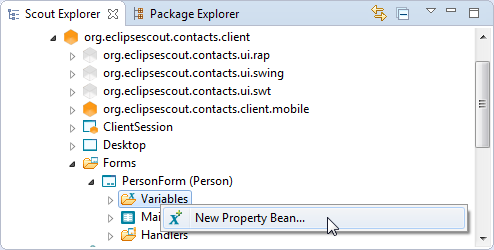
\includegraphics[height=4.5cm]{new_bean_personid_contextmenu.png} \hspace{5mm}
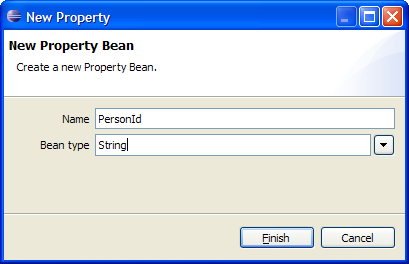
\includegraphics[height=4.5cm]{new_bean_personid.png}
\caption{Add the \element{PersonId} variable to the person form.}
\figlabel{new_bean_personid}
\end{figure}

To hold the persons primary key in the person form we also need to add a corresponding variable. 
For this, use the \wizard{New Property Bean} as shown in \figref{new_bean_personid}. 
In the wizard dialog, enter ''PersonId'' into the \field{Name} and pick \java{String} from the dropdown list provided in the \field{Bean type}. 
Then, click the \button{Finish} to close the wizard. 

% ........................................................................... %
\subsection{Creating the Form Layout with From Fields}

\begin{figure}
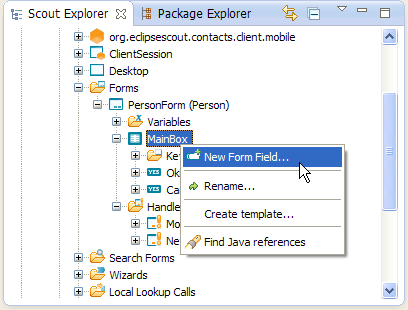
\includegraphics[width=7cm]{new_field_personbox.png} \hspace{5mm}
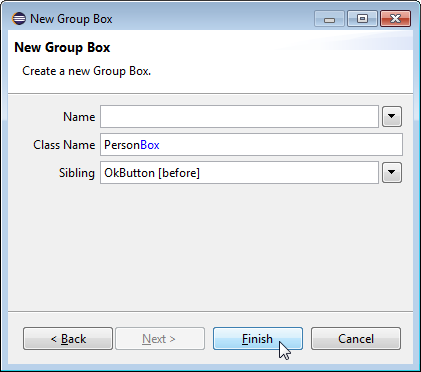
\includegraphics[width=7cm]{new_field_personbox_name.png}
\caption{Add the first group box field to the person form.}
\figlabel{new_field_personbox}
\end{figure}

As a next step we create the main layout structure of the person form. 
According to the screenshot of the person form shown in \figref{my_contacts_swt} the form is organized into an upper box including the first name, the last name and a picture field. 
In the ''Details'' box in the lower half of the form some additional fields are found, such as the date of birth field. 
The bottom of the form holds a ''Show Map ...'' link.
We start with the general layout by adding the \java{PersonBox} according to \figref{new_field_personbox}. 
And again on the person's from \node{MainBox} we add a second group box field using the label ''Detail''. 
The link is added with the \wizard{New Form Field} too. 
In the first wizard step select the type \java{LinkButton} and use a new translated text ''Show Map ...'' for the \field{Name}

We now add the form fields listed below using the the \wizard{New Form Field} multiple times. 
Most fields are of type \java{StringField} and different field types are separately indicated. 

\begin{itemize}
  \item{PersonBox}
  \begin{itemize}
    \item ''First Name'' 
    \item ''Last Name''
    \item PictureUrlField
    \item PictureField (ImageField)
  \end{itemize} 
  \item{''Detail'' DetailBox}
  \begin{itemize}
    \item ''Headline'' 
    \item ''Location''
    \item ''Date of Birth'' (DateField)
  \end{itemize} 
\end{itemize} 

\begin{figure}
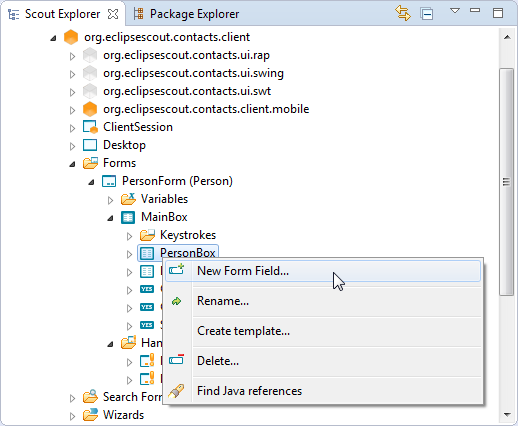
\includegraphics[width=7cm]{new_field_picture_contextmenu.png} \hspace{5mm}
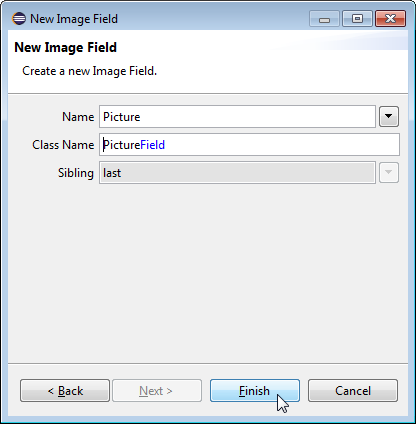
\includegraphics[width=7cm]{new_field_picture.png}
\caption{Add the picture field to the first group box of the person form.}
\figlabel{new_field_picture}
\end{figure}

As an example for adding the form fields, the process is illustrated in \figref{new_field_picture} for the creation of the picture field. 
In the field list we need to set non default properties for the \field{PictureUrlField} and the \field{PictureField}. 
The picture URL field will hold an URL pointing to the picture of the person to be displayed. 
As in the person form only the picture is to be displayed but not the picture URL, we need to make this field invisible. 
For this, select the \node{PictureUrlField} in the Scout Explorer and then untick the \field{Visible} in the Scout Object Properties. 
Note that to access the visibility property you need to open the section \element{Advanced Properties} first. 

\begin{figure}
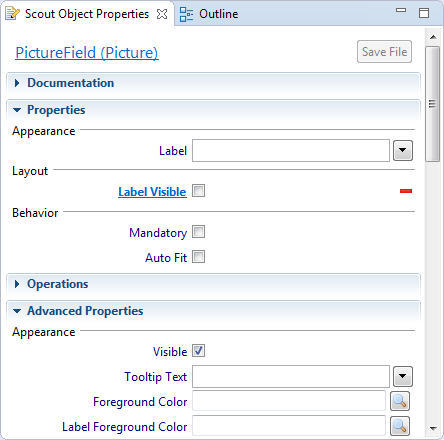
\includegraphics[width=7cm]{picture_field_properties_1.png} \hspace{5mm}
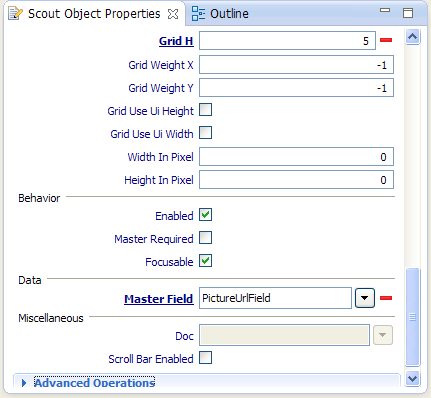
\includegraphics[width=7cm]{picture_field_properties_2.png}
\caption{Set the properties for the picture field of the person form.}
\figlabel{picture_field_properties}
\end{figure}

As the configuration of the picture field is more complex than the other fields, the changed properties are shown in the screenshots provided in \figref{picture_field_properties}. 
First, no label is shown for the picture field as shown in the unticked \field{Label Visible} of the Scout Object Properties. 
Then, property \element{Grid H} is set to 5. 
This results in the picture to cover the vertical space of 5 form fields. 

\lstinputlisting[
  label=\lstlabel{mycontacts.client.forms.person.picturefield},
  caption=The behaviour of the person form's \java{PictureField} is triggered by changes in field \java{PictureUrlField}.,
  index={getConfiguredMasterField, execChangedMasterValue, IOUtility},
  linerange={133-135,151-167,186-187},
  float
]
{../code/oneDayTutorial/org.eclipsescout.contacts.client/src/org/eclipsescout/contacts/client/ui/forms/PersonForm.java}

Finally, we want the picture to be refreshed whenever the content of the picture URL is changed. 
For this, the property \element{Master Field} is set to the \java{PictureUrlField}. 
The implementation of the corresponding method \java{execChangedMasterValue} is provided in \lstref{mycontacts.client.forms.person.picturefield}. 
As we can see, the Scout helper class \java{IOUtility} is used to read the image content from the provided URL. 
This content is then used to assign the image content with the image field's method \java{setImage}. 
Method \java{setAutoFit} is called to adapt the picture to the dimensions available to the image field. 

% ........................................................................... %
\subsection{A simple Form to edit the Picture URL}

\begin{figure}
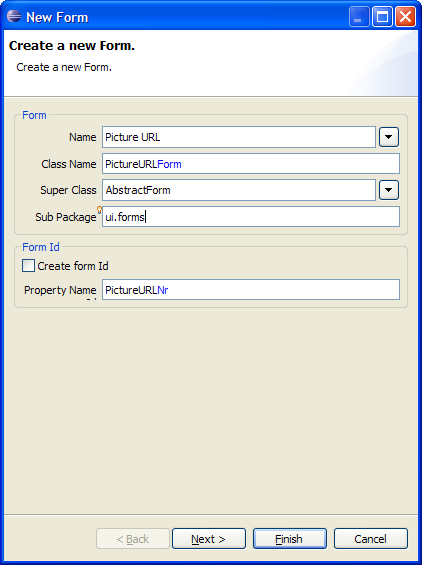
\includegraphics[width=7cm]{new_form_url_1.png} \hspace{5mm}
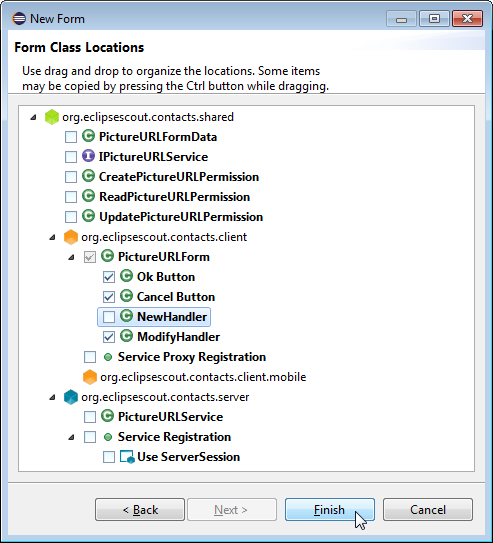
\includegraphics[width=7cm]{new_form_url_2.png}
\caption{Add the URL editor form.}
\figlabel{new_form_url}
\end{figure}

To edit a person's picture link, we create a simple URL editor form as shown in \figref{new_form_url}. 
As we only need this form to update the URL information of a person's picture field, we do not need any connectivity to the backend of the ''My Contacts'' application. 
That is why almost all form and service artefacts are deselected in the second wizard step shown on the right side of \figref{new_form_url}. 

\lstinputlisting[
  label=\lstlabel{mycontacts.client.forms.pictureurl},
  caption=The UI structure of the \java{PictureURLForm} used to update the URL of the picture field in the person form. The rest of the class created by the Scout SDK has been omitted.,
  linerange={17-18,52-67,78-80},
  float
]
{../code/oneDayTutorial/org.eclipsescout.contacts.client/src/org/eclipsescout/contacts/client/ui/forms/PictureURLForm.java}

As this form only holds a single URL field, we omit the description of the creation of the URL editor form's content and provide the resulting Java code instead. 
In \lstref{mycontacts.client.forms.pictureurl} just the form's \java{MainBox} code is shown. 

\begin{figure}
\includegraphics[width=7cm]{new_menu_editurl_contextmenu.png} \hspace{5mm}
\includegraphics[width=7cm]{new_menu_editurl.png}
\caption{Add the URL edit menu to the picture field.}
\figlabel{new_menu_editurl}
\end{figure}

This form is then started via an ''Edit URL ...'' contextmenu on the image field.
The creation of this contextmenu is shown in \figref{new_menu_editurl}. 
See \lstref{mycontacts.client.forms.person.picturefield.editmenu} for the actual implementation of the \java{execAction} for this contextmenu.

\lstinputlisting[
  label=\lstlabel{mycontacts.client.forms.person.picturefield.editmenu},
  caption=The edit menu implemented in class \java{EditURLMenu} of the picture field.
  If the URL was changed the picture URL field of the person form is set accordingly in method \java{execAction},
  index={execAction},
  linerange={168-185},
  float
]
{../code/oneDayTutorial/org.eclipsescout.contacts.client/src/org/eclipsescout/contacts/client/ui/forms/PersonForm.java}

Once the edit URL form is started with \java{form.startModify()} the client waits in method \java{form.waitFor} until the form is closed by the user. 
If the user has changed any field content (the picture URL in our case) and closed the form with the \button{OK}, the method \java{form.isFormStored} returns true, and we can copy the new URL from the editor form field into the picture URL field of the person form. 
Such a change will then trigger method \java{execChangedMasterValue} of the \java{PictureField} which in turn updates the image shown in the person form. 

% ........................................................................... %
\subsection{Linking the Person Form to the Person Page}

\begin{figure}
\includegraphics[width=7cm]{new_menu_editperson_contextmenu.png} \hspace{5mm}
\includegraphics[width=7cm]{new_menu_editperson.png}
\caption{Add the Person edit menu to the person page.}
\figlabel{new_menu_editperson}
\end{figure}

\lstinputlisting[
  label=\lstlabel{mycontacts.desktop.outline.personpage.editmenu},
  caption=The \java{EditPersonMenu} to edit the person selected in the person table.
  The person id taken from the corresponding (invisible) column is transferred to the person form before the form is started.,
  index={isFormStored, reloadPage},
  linerange={112-131},
  float
]
{../code/oneDayTutorial/org.eclipsescout.contacts.client/src/org/eclipsescout/contacts/client/ui/desktop/outlines/pages/PersonTablePage.java}

The user of the ''My Contacts'' application wants to use the person form to show/edit attributes of a specific person.
To support this use case, we need to link this form with the ''My Contacts'' application. 
As we already have person pages that show some of the person's attribute, we can now add context menus to this list to open/edit existing persons in the person form and to create new persons as well. 
This is achieved by using the \wizard{New Menu} on the \node{Menus} of the table of the person page according to \figref{new_menu_editperson}. 
In the \field{Name} enter the new translated text ''Edit Person ...''. 
The form to start is the \java{PersonForm} and the \java{ModifyHandler} is the form handler to be used to start the form. 
As we have defined a meaningful primary key column on the person page and a matching variable is available for the person form, the Scout SDK wizard is generating the necessary code automatically. 
The implementation of the \java{execAction} method provided in \lstref{mycontacts.desktop.outline.personpage.editmenu} works out of the box and should not need any manual tuning.
Now, you may also add the ''New Person ...'' menu in the same way. 
Except that you pick the \java{NewHander} in the \wizard{New Menu} instead of the modify handler. 

\begin{figure}
\includegraphics[height=5.5cm]{person_table_explorer.png} \hspace{5mm}
\includegraphics[height=5.5cm]{person_table_properties.png}
\caption{Set the behaviour for the row level action on the person table.}
\figlabel{person_table_properties}
\end{figure}

\lstinputlisting[
  label=\lstlabel{mycontacts.desktop.outline.personpage.execrowaction},
  caption=The \java{execRowAction} method on table pages is used to trigger an action when a row is selected with a double click or \textsc{<Enter>}.,
  index={execRowAction},
  linerange={58-62},
  float
]
{../code/oneDayTutorial/org.eclipsescout.contacts.client/src/org/eclipsescout/contacts/client/ui/desktop/outlines/pages/PersonTablePage.java}

To open the person form with a double click on a person row or by hitting the \key{Enter} key, you may add a corresponding \java{execRowAction} on the person page. 
This method can be added to the person table by clicking on the green plus icon next to the operation \element{Exec Row Action} as shown in \figref{person_table_properties}. 
For the implementation of this method you may reuse the functionality implemented for the context menu according to \lstref{mycontacts.desktop.outline.personpage.execrowaction}. 

% ........................................................................... %
\subsection{Adding the Company Smartfield}

At the current stage of the ''My Contacts'' application, we have no option to manage the relationship between people and companies. 
To manage this relation, we now add a company smartfield to the person form. 
This smartfield will then hold the current assignment of the person represented in the person form. 

A Scout smartfield can be viewed as user friendly dropdown field on steroids that also implements \element{search-as-you-type} to pick a specific entry. 
In the simplest case the smartfield provides access to a small and locally provided list of key value pairs. 
But for the intended use in the ''My Contacts'' application, we will need to access a list of elements provided by the server that will be compiled dynamically at runtime. 

\begin{figure}
\includegraphics[width=6cm]{new_lookupcall_company_contextmenu.png} 
\caption{Add a lookup call to the applications shared node.}
\figlabel{new_lookupcall_company_contextmenu}
\end{figure}

\begin{figure}
\includegraphics[height=5.5cm]{new_lookupcall_company_1.png} \hspace{5mm}
\includegraphics[height=5.5cm]{new_lookupcall_company_2.png}
\caption{The two wizard steps to enter the details of the company lookup call.}
\figlabel{new_lookupcall_company}
\end{figure}

To create the access to this list, we start with the creation of the company lookup call. 
As shown in \figref{new_lookupcall_company_contextmenu} the lookup call is added on the \folder{Lookup Calls} under the green shared node of the ''My Contacts'' application.
This opens the \wizard{New Lookup Call} as shown in \figref{new_lookupcall_company}. 
In the first wizard step, enter ''Company'' into the \field{Class Name} and verify that the wizard step looks the same as the screenshot shown on the left hand side of \figref{new_lookupcall_company}.
Before the wizard is closed, click on the \button{Next} to move to the second wizard step. 
As shown on the right hand side of \figref{new_lookupcall_company} the wizard will also create a corresponding \java{CompanyLookupService} on the application's server. 
We can now close this wizard with the \button{Finish}.

\lstinputlisting[
  label=\lstlabel{mycontacts.shared.lookup.companylookupcall},
  caption=The company lookup call with its \java{getConfiguredService} method in the application's shared plugin.,
  index={LookupCall, getConfiguredService, CompanyLookupCall},
  linerange={7-16},
  float
]
{../code/oneDayTutorial/org.eclipsescout.contacts.shared/src/org/eclipsescout/contacts/shared/services/lookup/CompanyLookupCall.java}

\lstinputlisting[
  label=\lstlabel{mycontacts.server.lookup.companylookupservice},
  caption=The company lookup service in the application's server plugin.
  The \java{key} and the \java{text} criteria are used to search for values by key or by the provided name substring.
  index={AbstractSqlLookupService, getConfiguredSqlSelect},
  linerange={6-20},
  float
]
{../code/oneDayTutorial/org.eclipsescout.contacts.server/src/org/eclipsescout/contacts/server/services/lookup/CompanyLookupService.java}

The \java{CompanyLookupCall} just created by the Scout SDK wizard is provided in \lstref{mycontacts.shared.lookup.companylookupcall}. 
As we can see, the only method implemented is \java{getConfiguredService} that points to the specific server service to be used. 
In the Scout Explorer, the new company lookup service can be found in the \folder{Lookup Services} under the blue server node of the application. 
In this service, we need to implement method \java{getConfiguredSqlSelect} as shown in \lstref{mycontacts.server.lookup.companylookupservice}. 
For Scout lookup services, specific \element{key}, \element{text} and \element{all} criteria blocks need to be provided. 
This criteria are included in the \java{SELECT} statement using the \java{<key>}, \java{<text>} and \java{<all>} tags as shown in the listing. 
The Scout runtime uses the \java{<key>}-block in cases where a specific key is already assigned to the smartfield. 
The \java{<text>}-block is used as a query criteria to create the dynamic \element{search-as-you-type} hit list based on the (sub)string entered by the user so far.
Finally, the \java{<text>}-block is used to define the hit list to be shown when the user does not enter any text into the smartfield but clicks on the field's search icon instead. 
The bind variable \java{:key} and \java{:text} are provided by Scout and hold the value of the assigned key or the text entered into the smartfield. 

\begin{figure}
\includegraphics[width=7cm]{new_smartfield_company_contextmenu.png}
\caption{Add a smartfield to the person form.}
\figlabel{new_smartfield_company_contextmenu}
\end{figure}

\begin{figure}
\includegraphics[height=5cm]{new_smartfield_company_1.png} \hspace{5mm}
\includegraphics[height=5cm]{new_smartfield_company_2.png}
\caption{Create the company smartfield for the person form.}
\figlabel{new_smartfield_company}
\end{figure}

We are now ready to add the company smartfield to the person form. 
To start the \wizard{New Form Field} we use the context menu on the \java{DetailBox} of the person form as shown in \figref{new_smartfield_company}.
In the first wizard step, we chose the \element{SmartField} entry as the field type and click the \button{Next}. 
Then, we enter ''Company'' into the \field{Name} as shown on the right hand side of \figref{new_smartfield_company}. 
Make sure that you select the \element{String} entry in the \field{Generic Type} as we are using string values to identify companies in the ''My Contacts'' application. 
And in the \field{LookupCall}, we can now select the \element{CompanyLookupCall} that we have just created before. 
Finally, the position of the new company smartfield can be set in the \field{Sibling} before the location field before the wizard is closed with the \button{Finish}. 

\lstinputlisting[
  label=\lstlabel{mycontacts.client.forms.person.companyfield},
  caption=The smartfield \java{CompanyField} of the person form and its wiring with the company lookup call.,
  index={AbstractSmartField, getConfiguredLookupCall},
  linerange={233-247},
  float
]
{../code/oneDayTutorial/org.eclipsescout.contacts.client/src/org/eclipsescout/contacts/client/ui/forms/PersonForm.java}

The implementation of the company smartfield created by the Scout SDK wizard is provided in \lstref{mycontacts.client.forms.person.companyfield}. 
A look at the implementation of the \java{CompanyField} class shows its simplicity and the wiring with the company lookup service.

% ........................................................................... %
\subsection{Adding the Map Form}

We now want to add the ''Map'' form shown in the front of \figref{my_contacts_swt}.
The purpose of this form is to show a map corresponding to the address entered into the \field{location} of the person form using the Google Maps Image API\footnote{
The Google Maps Image API can be used to fetch static map images: \url{https://developers.google.com/maps/documentation/imageapis/}.
}.
This also implies that only addresses that can correctly be parsed by the Maps Image API will lead to a useful map image.

To create the maps form we start the \wizard{New Form} and enter the new translated text ''Map'' into the \field{Name} of the first wizard step. 
Then, we click the \button{Next} to configure the artefacts to be created by the wizard. 
For the map form we can use the configuration as shown on the right hand side of \figref{new_form_url} with the difference that we do not need the Ok button.
Having deselected most artefacts, the wizard can be closed with the \button{Finish}.

After the form creation wizard has been closed, update the label of the cancel button to ''Close'' in the button's Scout Object Properties. 
Then, we can add an ''Address'' variable to the form by starting the \wizard{New Property Bean} on the \node{Variables} of the newly created map form.
In the property bean wizard, enter ''Name'' into the \field{Name} and set the \field{Bean type} to \element{String}. 

As the next step, the map image field is added to the from. 
For this, start the \wizard{New Form Field} directly on the form's \node{MainBox}. 
In the first form field wizard step, select \element{ImageField} as the field type and click on the \button{Next}. 
Before you can close the second wizard step with the \button{Finish}, enter ''Map'' into the \field{Class Name}. 
To set the properties of the new map field, select the \node{MapField} below the main box node of the map form. 
In the \java{MapField}'s Scout Object Properties untick the \property{Label Visible} and add an \java{execInitField} method by clicking on the green plus icon next to this operation. 
The configuration of the map field can then be completed in section \element{Advanced Properties}. 
Here, we set the \property{Grid H} to 6 and update the \property{Width in Pixel} and the \property{Height in Pixel} to a value of 400 each. 


\lstinputlisting[
  label=\lstlabel{mycontacts.client.forms.map},
  caption=In the \java{execInitField} method of the map form the image content is fetched from the Google Maps API.,
  index={execInitField, AbstractImageField},
  linerange={81-99},
  float
]
{../code/oneDayTutorial/org.eclipsescout.contacts.client/src/org/eclipsescout/contacts/client/ui/forms/MapForm.java}

To add the Java code to display the map in the image field, click on the \link{execInitField} in the Scout Object Properties of the map field. 
According to the implementation provided in \lstref{mycontacts.client.forms.map}, an URL for the Maps Image API is first constructed. 
This URL also contains the content of the map form's address variable and the configured dimension of the map field. 
The map picture returned by the Google API is then read using \java{IOUtility.getContent} and directly fed into the image fields \java{setImage} method. 

The last step involving the implementation of the map form feature is its integration into the person form. 
As visible on the lower left part of the person form shown in \figref{my_contacts_swt}, a \link{Show Map ...} is available. 
We now need to add such a link to the person form and add the necessary wiring for opening the newly created map form if the user clicks on this link. 
As a first step, the \wizard{New Form Field} is started on the \node{MainBox}. 
In the first wizard step, select the \element{LinkButton} from the available field types and click the \button{Next} to load the second wizard step. 
Here, just enter the new translated text ''Show Map ...'' into the \field{Name} and close the wizard with the \button{Finish}. 

\lstinputlisting[
  label=\lstlabel{mycontacts.client.forms.person.clickmaplink},
  caption=The edit menu implemented in class \java{EditURLMenu} of the picture field.
  If the URL was changed the picture URL field of the person form is set accordingly in method \java{execAction},
  index={execClickAction},
  linerange={275-290},
  float
]
{../code/oneDayTutorial/org.eclipsescout.contacts.client/src/org/eclipsescout/contacts/client/ui/forms/PersonForm.java}

To add the necessary wiring code to the link button double click the \node{ShowMapButton} in the Scout Explorer and implement its \java{execClickAction} method.
As shown in \lstref{mycontacts.client.forms.person.clickmaplink}, we only need to create a new map form in the click action, set its address variable and open the form with \java{form.startModify}.

% --------------------------------------------------------------------------- %
\section{Managing Person Data on the Server Side}

\lstinputlisting[
  label=\lstlabel{mycontacts.client.personform.modifyhandler},
  caption=The \java{execLoad} and the  \java{execStore} methods of the person form's modify handler.,
  index={ModifyHandler,AbstractFormHandler},
  linerange={292-312},
  float
]
{../code/oneDayTutorial/org.eclipsescout.contacts.client/src/org/eclipsescout/contacts/client/ui/forms/PersonForm.java}

In the ''My Contacts'' client application the person form is started via two separate form handlers called by the person page context menus. 
The new handler is used to start the form in the mode to create new persons while the modify handler is implemented to start the form for updating existing persons. 
When we look at the implementation of the modify handler provided in \lstref{mycontacts.client.personform.modifyhandler}, we see the two methods \java{execLoad} and \java{execStore}. 

As already described in \secref{helloworld.formhandler} of the ''Hello World'' tutorial, \java{execLoad} is called by the Scout framework the the form is started. 
Similarly, method \java{execStore} is called by the Scout framework after the user has clicked the \button{OK} of a form. 
In both methods, a corresponding service operation of the \java{PersonService} is called. 
From the form handler's \java{execLoad} method the method \java{load} of the person service is called. 
And the form handler's \java{execStore} method calls the person service's method \java{store} as shown in \lstref{mycontacts.server.services.personservice.load}. 

\lstinputlisting[
  label=\lstlabel{mycontacts.server.services.personservice.load},
  caption=The \java{load} and the \java{store} methods of the server's \java{PersonService}.,
  index={PersonService},
  linerange={18-19,48-96},
  float
]
{../code/oneDayTutorial/org.eclipsescout.contacts.server/src/org/eclipsescout/contacts/server/ui/forms/PersonService.java}

For the \java{load} method in \lstref{mycontacts.server.services.personservice.load} it is assumed that the in the provided parameter \java{formData} the person's id is available as a search criteria. 
It might be interesting to note that for the SQL \java{SELECT} and \java{UPDATE} statements we can provide the complete form data to use Scout's support for bind variables. 

The implementation of the person form's new handler is implemented similar to it's modify handler. 
Instead of calling the service operations \java{load} and \java{store}, the methods  \java{prepareCreate} and \java{create} are used. 
In principle, method \java{prepareCreate} is not needed for the ''My Contacts'' application. 
As its implementation has been created by the Scout SDK wizard, it does not any harm when the method is left as it is. 

\lstinputlisting[
  label=\lstlabel{mycontacts.server.services.personservice.create},
  caption=The \java{create} method of the server's \java{PersonService}.,
  index={PersonService},
  linerange={18-19,28-47,95-96},
  float
]
{../code/oneDayTutorial/org.eclipsescout.contacts.server/src/org/eclipsescout/contacts/server/ui/forms/PersonService.java}

In \lstref{mycontacts.server.services.personservice.create} the implementation of the \java{PersonService}'s \java{create} method is provided. 
First, the implementation checks if the provided form data contains a person id. 
If the person has been entered manually a value for this id is missing and a new id is provided using \java{formData.setPersonId(UUID.randomUUID().toString())}.
The only responsibility of the \java{INSERT} statement following the person id check is to make sure we will have a row in the \java{PERSON} table for the person to be created. 
To save all other form data parameters, we just need to call the previously implemented \java{store} method. 


% --------------------------------------------------------------------------- %
\section{Creating the Company Form}

Creating the company form and the necessary backend services is not described here.
Instead this task is left as an exercise to the reader and in the text below some minimal guidelines are provided.

The main trick is to start with the \wizard{New Form} to create the company form. 
This will create all necessary artefacts including the forms, necessary server services, and communication between the client and the server. 
Then, make sure you don't forget to add a variable \java{companyId} to the company form. 
To decide on the fields that need to be on the company form you may check the setup of the database schema provided in \lstref{mycontacts.server.services.installdb.company}. 
If in doubt about what to do, please refer to the procedure used to create the person form. 

In case you get lost completely, you may download the ''My Contacts'' application from this books Github repository as described in the Scout wiki\footnote{
Download and installation of the ''My Contacts'' application: \url{http://wiki.eclipse.org/Scout/Book/3.9\#Download_and_Run_the_Scout_Sample_Applications}.
}.

% --------------------------------------------------------------------------- %
\section{Adding the Scribe Library to the Application}

To access data from sites such as LinkedIn, Xing, Google+ or Facebook, most social networks provide an API that requires user authentication. 
The current defacto standard for such authentication is the Open Authentication Protocol (OAuth)\footnote{
For more information regarding the OAuth standard, see: \url{http://oauth.net/}.
} 

The big advantage of the OAuth standard is the access token based authentication. 
If an application such as the ''My Contacts'' example is in possession of an access token, it can fetch data from the hosting site or even act on the users behalf. 
It is important to note that the access token is just constructed of two values, the token and the secret.
And both values are completely separate from the user's username and password credentials. 
This means that an access token may be safely stored in other applications. 
Should such an application's data get compromised, the username and password are still save.
The user then has the option to remove the compromised access token.  

For the ''My Contacts'' application we use the Scribe Java library\footnote{
The Scribe OAuth Java library: \url{https://github.com/fernandezpablo85/scribe-java}.
}
This library makes accessing social services very simple.
At the same time the Scribe library is used here to demonstrate the integration of external Java libraries in Scout applications. 

\begin{figure}
\includegraphics[width=7cm]{new_library_scribe_contextmenu.png} \hspace{5mm}
\caption{Add a new bundle to hold the Scribe JARs.}
\figlabel{new_library_scribe_contextmenu}
\end{figure}

\begin{figure}
\includegraphics[width=7cm]{new_library_scribe_1.png} \hspace{5mm}
\includegraphics[width=7cm]{new_library_scribe_2.png}
\caption{Specify the JARs to be contained in the library bundle and the library name.}
\figlabel{new_library_scribe}
\end{figure}

As we will use the Scribe library only on the Scout server side start the Scout SDK \wizard{New Library Bundle} below the blue server node as shown in \figref{new_library_scribe_contextmenu}. 
In the first wizard step shown on the left side of \figref{new_library_scribe} add the files \filename{scribe-1.3.0.jar} and \filename{commons-codec-1.8.jar}\footnote{
See the getting started page for more information regarding the two necessary JAR file: \url{https://github.com/fernandezpablo85/scribe-java/wiki/getting-started}.
} 
using the \button{Add}. 
Once the two JAR files are listed in the library list of the wizard click the \button{Next}.
On the second wizard step, enter ''org.scribe'' into the \field{Bundle Name} as shown on the right side of \figref{new_library_scribe}. 
Then, close the wizard with the \button{Finish}.

The Scout SDK wizard then creates the corresponding library plugin and updates the server product files and the plugin dependencies of the applications server plugin accordingly. 
Once the wizard has completed the classes defined in the two JAR files can directly be accessed from the ''My Contact'' application's server plugin.

% --------------------------------------------------------------------------- %
\section{Integrating LinkedIn Access with Scribe}

\lstinputlisting[
  label=\lstlabel{mycontacts.server.linkedin.initialize},
  caption=The \java{LinkedInService} service with it's \java{initializeService} method defined in the \java{IService} interface.,
  index={IService, initializeService},
  linerange={32-50,160-161},
  float
]
{../code/oneDayTutorial/org.eclipsescout.contacts.server/src/org/eclipsescout/contacts/server/services/LinkedInService.java}

To access the LinkedIn data with Scribe a separate service \java{LinkedInService} is created in the \folder{Services} under the blue server node. 
Before we add any service operations to the LinkedIn service, the service initialization method is implemented according to \lstref{mycontacts.server.linkedin.initialize}. 
This initialization is not discussed further here.
Instead, the interested reader is referred to the corresponding \java{LinkedInExample} on the Scribe web pages\footnote{
For the Scribe \filename{LinkedInExample.java} example class see: \url{https://github.com/fernandezpablo85/scribe-java/blob/master/src/test/java/org/scribe/examples/LinkedInExample.java}.
}.

\begin{figure}
\includegraphics[height=5.5cm]{new_operation_authurl_contextmenu.png} \hspace{5mm}
\includegraphics[height=5.5cm]{new_operation_authurl.png}
\caption{Add the operation to retrieve an authentication URL.}
\figlabel{new_operation_authurl}
\end{figure}

\lstinputlisting[
  label=\lstlabel{mycontacts.server.linkedin.authurl},
  caption=The \java{getAuthUrl} method of the LinkedIn service.,
  index={AbstractSmartField, getConfiguredLookupCall},
  linerange={51-57},
  float
]
{../code/oneDayTutorial/org.eclipsescout.contacts.server/src/org/eclipsescout/contacts/server/services/LinkedInService.java}

The first service operation \java{getAuthUrl} is added according to \figref{new_operation_authurl}. 
This operation will return the necessary information to create a request token and provides a link to open in a web browser to start the authentication against the LinkedIn account. 
For its implementation see \lstref{mycontacts.server.linkedin.authurl}.

\begin{figure}
\includegraphics[height=5.5cm]{new_operation_refreshtoken.png} \hspace{5mm}
\includegraphics[height=5.5cm]{new_operation_updatecontacts.png}
\caption{Add the operations to refresh the access token and to update the LinkedIn contacts.}
\figlabel{new_operation_refresh_update}
\end{figure}

\lstinputlisting[
  label=\lstlabel{mycontacts.server.linkedin.refreshtoken},
  caption=The \java{refreshToken} method is used to create a new access token to fetch data from the LinkedIn API.,
  linerange={58-85},
  float
]
{../code/oneDayTutorial/org.eclipsescout.contacts.server/src/org/eclipsescout/contacts/server/services/LinkedInService.java}

The next operations we add are used to refresh the users access token stored in the ''My Contacts'' application and to refresh or download the users contacts stored in the user's LinkedIn account. 
See \figref{new_operation_refresh_update} for the necessary details for the creation of the two methods. 

Method \java{refreshToken} is implemented according to \lstref{mycontacts.server.linkedin.refreshtoken}. 
Using the provided token parameters and the security code, the access token is created using \java{m\_service.getAccessToken(...)}. 
Then, the user id of the currently logged in user is obtained with \java{ServerSession.get().getUserId()}. 
Once we have both the access token and the user id available in method {refreshToken}, we can store the token and the secret values for the current user in table \java{USERS\_PARAM} according to \lstref{mycontacts.server.linkedin.refreshtoken}.

In the current implementation of the ''My Contacts'' application this id will always be set to \java{anonymous}. 
The reason for this is the \java{AnonymousSecurityFilter} security filter that is activated during the initial project creation step. 
As for logging, and database access, the configuration of the security filters of the server application is defined in the server's \filename{config.ini} file.

\begin{lstlisting}[backgroundcolor=\color{white},language=ini]
org.eclipse.scout.http.servletfilter.security.AnonymousSecurityFilter#active=true
\end{lstlisting}

\lstinputlisting[
  label=\lstlabel{mycontacts.server.configini.securityfilter},
  caption=The default configuration of the basic security filter in the Scout server's \texttt{config.ini} file.,
  index={BasicSecurityFilter, config.ini},
  linerange={35-39},
  float
]
{../code/oneDayTutorial/org.eclipsescout.contacts.server/products/development/config.ini}

If you would like to change the ''My Contacts'' application to a multi-user setup, the next simpler option is to deactivate the anonymous security filter and use the basic security filter instead. 
In the server's \filename{config.ini} file the necessary config lines are already prepared as shown in \lstref{mycontacts.server.configini.securityfilter}. 
Just set \java{BasicSecurityFilter\#active=true} and ''My Contacts'' the client application will prompt you with a login dialog. 
In this dialog you may enter one of the login credentials specified in in the \java{BasicSecurityFilter\#users} parameter of the \filename{config.ini} file. 
To log in as user admin, enter password ''manager''. 
To add new users, just amend the \java{BasicSecurityFilter\#users} parameter with additional comma separated entries of the form \java{username\\\=password}.

\lstinputlisting[
  label=\lstlabel{mycontacts.server.linkedin.updatecontacts},
  caption=The \java{updateContacts} method is used to enter/update existing contacts based on new data fetched from LinkedIn.,
  linerange={86-122},
  float
]
{../code/oneDayTutorial/org.eclipsescout.contacts.server/src/org/eclipsescout/contacts/server/services/LinkedInService.java}

The implementation of service method \java{updateContacts} of the LinkedIn service is provided in \lstref{mycontacts.server.linkedin.updatecontacts}.
First, a service reference is obtained to the person process service. 
Then, the LinkedIn contacts obtained by method \java{readContacts} are stored in a \java{persons} list object. 
For each person, a form data is created and its person id parameter is set to \java{DomUtility.getValue(person, "id")}. 
Using the \java{load} method of the person process service all attributes of the person are loaded from the server's database. 
The new attribute values obtained from the corresponding LinkedIn contact are then used to update the corresponding form data parameters. 
The newly updated person form data is then stored in the database with \java{service.create(formData)}.
Before we go through the \java{readContacts} method, we have a look at the explicit format of the contact data provided by the LinkedIn API. 

\begin{lstlisting}[
  label=\lstlabel{linkedin.samplexmlcontact},
  caption=A sample contact represented in the XML format provided by the LinkedIn API.,
  backgroundcolor=\color{white},
  language=xml,
  float
]
<?xml version="1.0" encoding="UTF-16"?>
<person>
    <id>f7R6wGcblj</id>
    <first-name>Mike</first-name>
    <last-name>Milinkovich</last-name>
    <headline>Executive Director at Eclipse Foundation</headline>
    <picture-url>http://m3.licdn.com/mpr/mprx/0_IUM7Se9vBU...SbRbQZ4</picture-url>
    <site-standard-profile-request>
      <url>http://www.linkedin.com/profile/view?id=14949387...05720*s114280*</url>
    </site-standard-profile-request>
    <location>
      <name>Ottawa, Canada Area</name>
      <country>
        <code>ca</code>
      </country>
    </location>
    <industry>Computer Software</industry>
  </person>
\end{lstlisting}

\lstinputlisting[
  label=\lstlabel{mycontacts.server.linkedin.domutil},
  caption=The \java{DomUtility} class provides functions to parse the XML data structure provided by the LinkedIn API.,
  linerange={13-45},
  float
]
{../code/oneDayTutorial/org.eclipsescout.contacts.server/src/org/eclipsescout/contacts/server/services/DomUtility.java}

From the sample XML extract provided in \lstref{linkedin.samplexmlcontact}, we can readily identify the person id \java{f7R6wGcblj}, the first name \java{Mike} and some other attribute names with associated attribute values. 
A closer look reveals the identity of the person to be Mike Milinkovich, a well known character in the Eclipse community. 
For each LinkedIn contact this format is parsed in method \java{readContacts} into a DOM tree\footnote{
DOM stands for Document Object Model. See \url{http://www.w3.org/DOM/} for more information.
}. 
Using the \java{DomUtility} helper class provided in \lstref{mycontacts.server.linkedin.domutil}, these attribute values are then extracted from this DOM tree and used to update the existing person attributes. 

\lstinputlisting[
  label=\lstlabel{mycontacts.server.linkedin.readcontacts},
  caption=The \java{readContacts} method to fetch the users connection using the LinkedIn API.
  The necessary access token is created in method \java{getToken} based on the information stored in the database for the logged in user.,
  linerange={123-159},
  float
]
{../code/oneDayTutorial/org.eclipsescout.contacts.server/src/org/eclipsescout/contacts/server/services/LinkedInService.java}

Accessing the user's LinkedIn contact list is implemented in method \java{readContacts} according to \lstref{mycontacts.server.linkedin.readcontacts}.
In this method, a signed OAuth request is first created using the access token provided by method \java{getToken}. 
The request specified by constant \java{LINKEDIN\_CONNECTIONS} is defined as \java{http://api.linkedin.com/v1/people/\textasciitilde/connections}. 
According to the API specification\footnote{
See the LinkedIn API documented for more specific information: \url{https://developer.linkedin.com/documents/linkedin-api-resource-map}.
} 
this returns all connections of the user.
To sign the request, the access token is retrieved from the database of the ''My Contact'' application using method \java{getToken}. 
According to the implementation provided in \lstref{mycontacts.server.linkedin.readcontacts} the user id is first obtained from the user's server session. 
The necessary parameters to create the access token are then retrieved from the \java{USERS\_PARAM} table. 
We have now implemented all necessary server services and operations to access the LinkedIn API, to create/refresh access tokens and to retrieve the users contacts. 

% --------------------------------------------------------------------------- %
\section{Fetching Contacts from LinkedIn}

\begin{figure}
\includegraphics[width=7cm]{new_form_token_1.png} \hspace{5mm}
\includegraphics[width=7cm]{new_form_token_2.png}
\caption{Add the form to refresh the LinkedIn access token.}
\figlabel{new_form_token}
\end{figure}

The last piece that is missing to complete the ''My Contacts'' application is the user interaction for the LinkedIn integration implemented in the previous section. 
To allow the user to create/refresh an access token, we need to implement the refresh token form shown in \figref{my_contacts_rayo_refresh} at the beginning of this chapter. 
To create the form code, we use the \wizard{New Form} of the Scout SDK as shown in \figref{new_form_token}. 
For the \field{Name} enter a new translated text ''Refresh LinkedIn Token'' and fill \java{ui.forms} into the \field{Sub Package} field. 
Then, click the \button{Next} to switch to the second wizard step. 
Here, deselect the elements that will not be needed for the implementation of the refresh form according to the right hand side of \figref{new_form_token}. 
Once the form has been created by the wizard, add the a \java{Token} and a \java{Secret} form variable of type string under the form's \folder{Variables}. 

\begin{figure}
\includegraphics[width=7cm]{tokenform_securitycode_explorer.png} \hspace{5mm}
\includegraphics[width=7cm]{tokenform_securitycode_properties.png}
\caption{The token form in the explorer and the properties of the security code field.}
\figlabel{tokenform_securitycode}
\end{figure}

The next step is to add the desired layout and the necessary form fields. 
First, use the \wizard{New Form Field} to add a new group box \java{TokenBox} to the \node{MainBox}. 
And into the \java{TokenBox} add a ''Security Code'' string field as shown on the left hand side of \figref{tokenform_securitycode}. 
To provide a click-able link that opens a web browser with the LinkedIn authentication link, add a ''Open Auth URL'' link of type \java{LinkButton} to the main box. 
To make the user to first click the authentication link button before he tries to fill any content into the security code field we initially disable this field. 
For this, first click on the security code field in the Scout Explorer and then open the \element{Advanced Properties} section of the fields Scout Object Properties. 
As shown on the right side of \figref{tokenform_securitycode}, deselect the \property{Enabled}.

\lstinputlisting[
  label=\lstlabel{mycontacts.client.forms.refreshtoken},
  caption=The structure of the refresh token form. The security code field gets enabled in method \java{execClickAction} after the authentication link button is pressed.,
  index={AbstractLinkButton,execClickAction},
  linerange={23-25,65-104},
  float
]
{../code/oneDayTutorial/org.eclipsescout.contacts.client/src/org/eclipsescout/contacts/client/ui/forms/RefreshTokenForm.java}

The implementation of the forms' structure is provided in \lstref{mycontacts.client.forms.refreshtoken}.
In the \java{execClickAction} method of the link button \java{OpenAuthURLButton} the necessary information for the auth link is obtained from the server. 
For this, we are using the \java{getAuthUrl} operation implemented in the previous section. 
The parameters to create the request token are saved in the form's token and secret variables. 
Then, the auth link is opened in a web browser with the \java{shellOpen}  method of the client's shell service. 
Finally, after opening the web browser we can enable the security field with \java{getSecurityCodeField().setEnabled(true)}.

\begin{figure}
\includegraphics[width=7cm]{new_menu_refreshtoken_contextmenu.png} \hspace{5mm}
\includegraphics[width=7cm]{new_menu_refreshtoken.png}
\caption{Add the menu to open the LinkedIn token form.}
\figlabel{new_menu_refreshtoken}
\end{figure}

We can now integrate the form to refresh the LinkedIn access token under the applications ''File'' menu. 
This is done using the \wizard{New Menu} as shown in \figref{new_menu_refreshtoken}. 
Enter the translated text ''Refresh LinkedIn Token ...'' into the wizard's \field{Name} and pick the element \element{Exit Menu [before]} from the dropdown box of the \field{Sibling}. 
In the \field{Form to start} select the newly created refresh token form and use the \element{NewHandler} entry in the \field{Form Handler}. 
To close the wizard, click the \button{Finish}.

\lstinputlisting[
  label=\lstlabel{mycontacts.client.desktop.refreshtokenmenu},
  caption=The menu to refresh the LinkedIn token starts the token form and then sends token parameters with the new security code to the LinkedIn backend service.,
  linerange={79-105},
  float
]
{../code/oneDayTutorial/org.eclipsescout.contacts.client/src/org/eclipsescout/contacts/client/ui/desktop/Desktop.java}

The implementation of the refresh menu is shown in \lstref{mycontacts.client.desktop.refreshtokenmenu}. 
In method \java{execAction()}, we need to amend the part after starting the refresh token form. 
If the method \java{form.isFormStored()} returns \java{true}, the user has modified the secure code field and it is fair to assume that the user wants to create/refresh his LinkedIn access token. 
For this, we first retrieve the necessary parameters to call the backend service operation \java{refreshToken} implemented in the previous chapter. 

\begin{figure}
\includegraphics[width=7cm]{new_menu_updatecontacts_contextmenu.png} \hspace{5mm}
\includegraphics[width=7cm]{new_menu_updatecontacts.png}
\caption{Add the menu to update the LinkedIn contacts.}
\figlabel{new_menu_updatecontacts}
\end{figure}

\lstinputlisting[
  label=\lstlabel{mycontacts.client.desktop.refreshtokenmenu},
  caption=The menu to update the stored persons with current LinkedIn data.,
  linerange={129-144},
  float
]
{../code/oneDayTutorial/org.eclipsescout.contacts.client/src/org/eclipsescout/contacts/client/ui/desktop/Desktop.java}

As the last missing component of the ''My Contacts'' application, we add the menu to fetch the LinkedIn contacts and update the database accordingly. 
The menu entry is created as a sub menu of the ''Tools'' menu.
For this, use the new menu wizard on the \node{ToolsMenu} as shown in \figref{new_menu_updatecontacts}. 
The implementation of the menu's \java{execAction} method shown in \lstref{mycontacts.client.desktop.refreshtokenmenu} is trivial. 
We only need to call the operation of the \java{LinkedInService} implemented in the server part of the ''My Contacts'' application. 

\ifx\wholebook\relax\else
   \begin{thebibliography}{99}
  \addcontentsline{toc}{chapter}{Bibliography}
  
  % add/insert books in alphabetical order of 1st author
  
  \bibitem{batessierra05}
    \textit{Bert Bates, Kathy Sierra},
	\textbf{Head First Java} 2nd edition, 
	O'Reilly Media, 2005.

  \bibitem{bloch08} 
    \textit{Joshua Bloch},
    \textbf{Effective Java} 2nd edition, 
	Addison-Wesley, 2008.
	
  \bibitem{eckel06}
    \textit{Bruce Eckel},
	\textbf{Thinking in Java} 4th edition, 
	Prentice Hall International, 2006.

\end{thebibliography}

   \end{document}
\fi

% =========================================================================== %
